\documentclass[letterpaper,11pt]{article}
\usepackage[english]{babel}
\usepackage[utf8]{inputenc}
\usepackage{tabularx} % extra features for tabular environment
\usepackage[margin=1in,letterpaper]{geometry} % decreases margins
\usepackage{cite} % takes care of citations
\usepackage[final]{hyperref} % adds hyper links inside the generated pdf file
\usepackage{graphicx}
\usepackage{amsmath}
\usepackage{amssymb}
\usepackage{subcaption}
\usepackage{hyperref}
\usepackage{caption}
\usepackage{graphicx}
\usepackage{booktabs}
\usepackage[toc,page]{appendix}
\graphicspath{ {./images/} }

% https://www.overleaf.com/project/5c33a36d705dd34ecb9180c2

\hypersetup{
	colorlinks=true,       % false: boxed links; true: colored links
	linkcolor=blue,        % color of internal links
	citecolor=blue,        % color of links to bibliography
	filecolor=magenta,     % color of file links
	urlcolor=blue         
}

\usepackage{Sweave}
\begin{document}
\Sconcordance{concordance:seminarska.tex:seminarska.Rnw:%
1 28 1 1 0 8 1 1 7 119 1 1 6 15 0 1 2 3 1 1 6 21 0 1 2 7 1 1 6 22 0 1 2 %
8 1 1 6 16 0 1 2 1 1 1 6 16 0 1 2 26 1 1 6 16 0 1 2 1 6 16 0 1 2 6 1}



\title{\Large{Predicting League of Legends match outcome with Bayesian methods}}
\author{Z. Nagelj}
\date{\today}
\maketitle


\section{Uvod}
Logistična regresijska se uporablja za analizo povezavo med kategorično odvisno spremenljivko in neodvisnimi  spremenljivkami.Polege logistične regresije se za analizo kategoričnih spremenljivk uporablja diskriminantna analiza, ki za razliko od logistične regresije predpostavlja normalno porazdelitev neodvisnih spremenljivk.


\section{Logistična regresija}
Kot vhodni podatek za logistično regresijo dobimo podatkovni set N točk. Vsaka i-ta točko sestavlja set m-tih neodvisnih spremenljivk in kategorična odvisna spremenljivka $Y_i$ z dvema možnima izidoma.


\subsection{Logit in logistična transormacija}
Naši kategorični odvisni spremenljivki najprej dodelimo numerične vrednost (0 in 1). Povprečje na vzorcu predstavlja delež ugodnih izidov \emph{p}, razmerje $p/(1-p)$ pa obeti (odds). Logit transormacijo  definiramo kot logaritem obetov (log odds):
$$l = logit(p) = \log{\frac{p}{1-p}} $$

\noindent S pomočjo te transformacije preidemo iz omejene zaloge vrednosti p na intervalu $[0,1]$, na obete $p/(1-p)$ omejene z zalogov vrednosti $[0, \infty)$ in na koncu na logaritem obetov z zalogo vrednosti $(-\infty, \infty)$. Inverzno transormacijo imenujemo logistična transformacija:
$$p = \text{logistic}(l)=\frac{\exp{l}}{1 + \exp{l}}$$

\noindent S transformacijo se izognemo problemu omejene zaloge vrednosti odvisne spremenljivke. Potencialno bi lahko izbrali tudi kakšno drugo transormacijo (probit).

\subsection{Logistični model}
Kategorično odvisno spremenljivko definiramo kot slučajno spremenljivko $Y_i$porazdeljeno po Bernoulliju s pričakovano vrednostjo $p_i$. Vsak izid je torej določen s svojo neznano verjetnostjo $p_i$, ki je določena na podlagi neodvisnih spremenljivk.
\newpage

$$Y_i | x_{1,i},...,x_{m,i}\sim \text{Bernoulli}(p_i)$$
$$E[Y_i | x_{1,i},...,x_{m,i}] = p_i$$
$$P(Y_i = y| x_{1,i},...,x_{m,i}) = p_i^y(1-p_i)^{(1-y)}$$


\noindent Ideja je zelo podobna kot pri linearni regressiji, torej verjetnost $p_i$ modeliramo kot linearno kombinacijo neodvisnih spremenljivk. Razlika je v tem, da verjetnosti transformiramo s pomočjo logit funkcije. V modelu nastopa dodaten intercept člen, zato imamo $m + 1$ regresijskih koficientov $\beta$.

$$\text{logit}(E[Y_i|X_i]) = logit(p_i) = \log{\frac{p_i}{1-p_i}} = X_i \beta$$

\noindent Oziroma:

$$E[Y_i|X_i] = p_i = \text{logit}^{-1}(X_i \beta) = \frac{1}{1+\exp^{-X_i \beta}}$$
$$P[Y_i = y_i|X_i] = p_i^y(1-p_i)^{1-y} = \frac{\exp^{y_i X_i \beta}}{1+\exp^{X_i \beta}}$$


\subsection{Določanje vrednosti regresijski koficientov}
Regresijski koficienti in verjetnosti $p_i$ so določene optimizacijo, na primer MLE. Za lažjo predstavo si najprej ogledamo MLE za enostaven primer Bernoullija:

\subsection{MLE za Bernoulli($p$)}
Zapišemo enačbo za verjetje in jo logaritmiramo. 
$$L = \prod_{i=1}^n p^{Y_i}(1-p)^{1-Y_i}=p^{\sum_{i=1}^n Y_i}(1-p)^{n-\sum_{i=1}^n Y_i}$$
$$l = \log{(L)} = \sum_{i=1}^n Y_i \log{(p)} + (n-\sum_{i=1}^n Y_i)\log{(1-p)}$$

\noindent Cenilko za $\hat{p}$ določimo s prvim parcialnim odvodom, ki ga enačimo z 0. Za asimptotski interval zaupanja cenilke določimo Fisherjevo informacijsko matriko. Saj populacijske vrednosti $p$ ne poznamo Fisherjevo informacijo določimo z oceno $\hat{p}$.

$$\hat{p}=\frac{1}{n}\sum_{i = 1}^n Y_i$$
$$I(p) = E[-\frac{\partial^2 l}{\partial p^2}]= \frac{1}{p(1-p)}$$
$$\hat{(var)} = \frac{1}{nI(\hat{p})} = \frac{\hat{p}(1-\hat{p})}{n}$$
$$\hat{(SE)} = \sqrt{\frac{\hat{p}(1-\hat{p})}{n}}$$

\noindent Za velik n je naša cenilka porazdeljena približno normalno:
$$\hat{p} \sim_{CLI} \text{Normal}(p, \frac{p(1-p)}{n})$$


\subsection{MLE za Bernoulli($p_i$)}
Saj ima pri logisicne regresije vsak izid svojo verjetnost $p_i$ je naša enačba za verjetje naslednja:

$$L = \prod_{i=1}^n p_i^{Y_i}(1-p_i)^{1-Y_i}=p_i^{\sum_{i=1}^n Y_i}(1-p_i)^{n-\sum_{i=1}^n Y_i} = 
(\frac{\exp^{X_i \beta}}{1+\exp^{X_i \beta}})^{\sum_{i=1}^n Y_i}(\frac{1}{1+\exp^{X_i \beta}})^{n-\sum_{i=1}^n Y_i}$$

$$l = \log{(L)} = \sum_{i=1}^n Y_i \log{(\frac{\exp^{X_i \beta}}{1+\exp^{X_i \beta}})} + (n-\sum_{i=1}^n Y_i)\log{(\frac{1}{1+\exp^{X_i \beta}})}$$

\noindent Posamezne regresijske koficiente dobimo s parcialnim odvodom logaritma verjetja. Saj rešitev v zaključeni formi ne obstaja uporabimo numeriče metode (npr. Newtnova metoda). Prav tako določimo informacijsko matriko za določanje asimptotske kovariančne matrike in intervalov zaupanja.


\section{Statistično testiranje regresijskih koficientov}
Za testiranje hipotez neničelnosti regresijski koficientov sta v uporabi Waldov test in  test razmerja verjetij.

\subsection{Waldov test}
Waldov test se uporablja za določanje statistične značilnosti posameznih regresijskih koficientov (podobno kot t-test pri linearni regresiji). Za koficiente pridobljene z MLE je testna statistika naslednja:
$$Z = \frac{\hat{\beta_i}}{\hat{SE}}$$

\noindent Ničelelna hipoteza testira $H_0: \beta_i =0$. Kot velja za vse cenilke pridobljene po metodi največjega verjetja so te asimptotsko nepristranske (dosledne) in normalno porazdeljene okoli prave vrednosti z varianco $\frac{1}{nI(p)}$.

\subsection{Test razmerja verjetij}
Pri testu nas zanima logaritem Wilksovega lambda pri dveh različnih modelih, pri čemer je en model gnezden (podmnožica drugega). Primerjali bomo polni model s \textbf{k} regresijskimi koficienti in delni model z \textbf{m} regresijskimi koficienti, kjer je $\textbf{m} < \textbf{k}$. Ničelna hipoteza (delni model) trdi da so testirani regresijski koficienti enaki 0. Alternativna hipoteza (polni model) pa trdi, da so vsi regresijski koficienti različni od 0. Pod ničelno hipotezeo torej testiramo ničelnost k - m $\beta$. Naša testrna statistika je:
$$LR = -2 \log{\Lambda} = -2 \log{\frac{L(H_0)}{L(H_A)}} = -2(l(H_0) - l(H_A))=-2(l(\hat{\beta}^{(0)}) - l(\hat{\beta}))$$
Asimptotsko je ta porazdeljena s $\chi^2$ z k - m stopinjami prostosti. Test razmerja verjetij se od Waldovega testa razlikuje po tem, da je potrebno narediti dva modela pod različnimi hipotezami.

\section{Naloga}
\subsection{Opis}
Na vzorcu bolnikov z rakom primerjamo dve vrsti operacije. Zanima nas ali obstaja povezanost s stadijem bolnika in ali ena vrsta operacije povzroča manj zapletov. Cilj naloge je analizirati napako I. reda pri testiranja hipotez na način, da testiramo vsako spremenljivko posebaj. 

\subsection{Postopek testiranje}
Sledili bomo naslednjim korakom:

\subsubsection{Stadij}
\begin{enumerate}
  \item Generiranje podatkov pod dano hipotezo
  \item Izdelava 4 modelov logistične regresije z informacijo o posameznem stadiju
  \item Pridobimo p-vrednosti Waldovega testa vseh 4 modelov z delnimi podatki
  \item Izdelava 1 modela logistične regresije z informacijo o vseh stadijh (1 spremenljivka)
  \item Pridobimo p-vrednosti testa razmerja verjetij za model z vsemi podatki
  \item Analiziramo porazdelitve p-vrednosti in primerjamo deleže zavrnjenih hipotez
\end{enumerate}

\subsubsection{Zaplet}
\begin{enumerate}
  \item Generiranje podatkov pod dano hipotezo
  \item Izdelava 10 modelov logistične regresije z informacijo o posameznem zapletu
  \item Izdelava 1 modela logistične regresije z informacijo o vseh zapletih (10 spremenljivk)
  \item Pridobimo p-vrednosti Waldovega testa vseh 11 modelov
  \item Analiziramo porazdelitve p-vrednosti in primerjamo deleže zavrnjenih hipotez
\end{enumerate}


\subsection{Pričakovani rezultati}
Zagotovo, pričakujemo, da bo naveden način testiranja pri stadiju napačen, saj so stadiji med seboj neodvisni, česar v modelih ne zajamemo. Prav tako v model ne vključimo informacije o ostalih stadijih in jih obravnavamo kot enakovredne. Pravilno bi stadij tako,  da ga v celoti vključimo v model ter z testom razmerja verjetij testiramo neničelnost regresijskega koficienta.

\noindent Pri obravnavi zapletov operacij, ob predpostavki da so si te neodvisni, predvidevam, da tak način testiranja ne bi bil napačen. V realnost pa temu zagotovo ni tako in so posamezni zapleti med seboj povezani, zato bi zagotovo naleteli na enake probleme kot pri testiranju posameznega stadija.

\section{Podatki}
\subsection{Generiranje}
Saj je v nalogi določeno, da je vzorec velik 300 pacientov, kjer vsaka polovica prejme en tip operacije, najprej generiramo večji vzorec $k=10000$ bolnikov iz katerga bomo vzorčili. Pridobiti moramo vrednosti spremenljivke stadij in desetih spremenljivk zaplet.

\subsubsection{Stadij}
Definiramo populacijske verjenosti za vsak stadij (Tabela~\ref{table:1}), ter glede na njih s funkcijo \emph{sample} izžrebamo stadij vsakega bolnika in določimo modelsko matriko. Verjetnosti stadijev se morajo sešteti v 1.

% latex table generated in R 3.5.1 by xtable 1.8-2 package
% Wed Apr 24 19:51:15 2019
\begin{table}[ht]
\centering
\begin{tabular}{rr}
  \hline
 & verjetnost \\ 
  \hline
Stadij 1 & 0.60 \\ 
  Stadij 2 & 0.25 \\ 
  Stadij 3 & 0.10 \\ 
  Stadij 4 & 0.05 \\ 
   \hline
\end{tabular}
\caption{Populacijski verjenosti posameznega stadija raka} 
\label{table:1}
\end{table}
\subsubsection{Zaplet}
Definiramo populacijske verjenosti za vsak zaplet (Tabela~\ref{table:2}), ter glede na njih s funkcijo \emph{rbinom} izžrebamo ali se je posamezen zaplet zgodil.

% latex table generated in R 3.5.1 by xtable 1.8-2 package
% Wed Apr 24 19:51:15 2019
\begin{table}[ht]
\centering
\begin{tabular}{rr}
  \hline
 & verjetnost \\ 
  \hline
Stadij 1 & 0.10 \\ 
  Stadij 2 & 0.12 \\ 
  Stadij 3 & 0.14 \\ 
  Stadij 4 & 0.16 \\ 
  Stadij 5 & 0.18 \\ 
  Stadij 6 & 0.20 \\ 
  Stadij 7 & 0.30 \\ 
  Stadij 8 & 0.40 \\ 
  Stadij 9 & 0.50 \\ 
  Stadij 10 & 0.60 \\ 
   \hline
\end{tabular}
\caption{Populacijski verjenosti posameznega zaplete pri operaciji} 
\label{table:2}
\end{table}

\subsubsection{Vzorec}
Ko imamo določene vrednosti spremenljiv na podlagi definirane hipoteze (oz. regresijskih koficientov) določimo linearne kombinacije spremenljivk ter s pomočjo logit transformacije verjetnost za tip operacije za vsakega izmed $k$ bolnikov. Izbran tip operacij pridobimo iz Bernoullijeve porazdelitve, glede na $p_i$. Da zadostimo specifikacijam naloge iz vzorca $10000$ bolnikov ob vsaki izmed $m=1000$ ponovitev naključno izžrebamo 150 operacij vsakega tipa.

\subsection{Hipoteze}
Podatke generiramo glede na 2 hipoteze, ničelno in alternativno. Glede na ničelno hipotezo so vsi regresijski koficienti enaki 0. Vrednosti regresijski koficientov pod alternativno hipotezo so vidni v Tabeli~\ref{table:3}.

% latex table generated in R 3.5.1 by xtable 1.8-2 package
% Wed Apr 24 19:51:15 2019
\begin{table}[ht]
\centering
\begin{tabular}{rrr}
  \hline
 & stadij & zaplet \\ 
  \hline
beta0 & 0.00 & 0.00 \\ 
  beta1 & 0.10 & -3.50 \\ 
  beta2 & 0.30 & 3.00 \\ 
  beta3 & 0.60 & -2.50 \\ 
  beta4 & -1.20 & 2.00 \\ 
  beta5 &  & -1.50 \\ 
  beta6 &  & 1.00 \\ 
  beta7 &  & -0.80 \\ 
  beta8 &  & 0.60 \\ 
  beta9 &  & -0.40 \\ 
  beta10 &  & 0.20 \\ 
   \hline
\end{tabular}
\caption{Vrednosti regresijski koficientov pri HA glede na neodvisno spremenljivko} 
\label{table:3}
\end{table}
\newpage
\section{Rezultati}
Opazujemo velikost testa (Tabela~\ref{table:4}, ~\ref{table:6}) in moč (Tabela~\ref{table:5}, ~\ref{table:7}). Notacija P(zavrneX) predstavlja delež zavrnjenih ničelnih hipotez glede na tip modela. U v predstavlja model, ko upoštevamao le informacije o posameznem stadiju/zapletu, M pa predstavlja model z vsemi informacijami. Iz simulacije smo določili še verjetnosti, da oba testa zavrneta Hipotezo, ter pogojne verjetnosti glede na kaj prikaže prvi test. 

V velikem številu raziskav si na tak način pomagamo pri izbiri neodvisnih spremenljivk. Torej za vsako izmed neodvisnih spremenljivk se izvede regresija in na podlagi tega določi katere spremenljivke bomo vključili v glavni model. Zato nas zanima s kašno verjetnostjo bomo spremenljivko s takšnim načinom pravilno izločili. To nam pove P(zavrneM | zavrneU). Velja seveda tudi obratno.
\subsection{Stadij}
Pri modeliranju posameznih stadijev, je v resnici naša ničelna hipoteza, da stadij_n nima vpliva na tip operacije, raziskovalno vprašanje pa se nanaša na stadij kot celota. Test je torej nesmiseln že z vidika raziskovalnega vprašanja. To se vidi tudi pri moči testa (Tabela~\ref{table:5}), kjer je moč pri pravem modelu v primerjavi z močjo posameznega modela precej večja, kot pri posameznih stadijih, še posebaj kjer je $\beta_S1$ blizu 0.

Vidimo, da če gledamo velikosti posameznih testov so vsi približno 0.05. Rezultati nam jasno povejo P(zavrneM | zavrneU), da s takšnim načinom modeliranja, v določenih primerih spremenljivke po krivem izključimo v tudi do 60\% primerih.
% latex table generated in R 3.5.1 by xtable 1.8-2 package
% Wed Apr 24 19:51:15 2019
\begin{table}[ht]
\centering
\begin{tabular}{rrrrr}
  \hline
 & S1 & S2 & S3 & S4 \\ 
  \hline
P(zavrneU) & 0.051 & 0.053 & 0.047 & 0.032 \\ 
  P(zavrneM) & 0.054 & 0.054 & 0.054 & 0.054 \\ 
  P(zavrneM $|$ zavrenU) & 0.377 & 0.396 & 0.389 & 0.509 \\ 
  P(zavrneU $|$ zavrenM) & 0.353 & 0.390 & 0.336 & 0.301 \\ 
   \hline
\end{tabular}
\caption{Verjetnosti zavrnitev pri H0} 
\label{table:4}
\end{table}

% latex table generated in R 3.5.1 by xtable 1.8-2 package
% Wed Apr 24 19:51:15 2019
\begin{table}[ht]
\centering
\begin{tabular}{rrrrr}
  \hline
 & S1 & S2 & S3 & S4 \\ 
  \hline
P(zavrneU) & 0.071 & 0.119 & 0.255 & 0.603 \\ 
  P(zavrneM) & 0.670 & 0.670 & 0.670 & 0.670 \\ 
  P(zavrneM $|$ zavrenU) & 0.938 & 0.931 & 0.942 & 0.874 \\ 
  P(zavrneU $|$ zavrenM) & 0.100 & 0.166 & 0.359 & 0.787 \\ 
   \hline
\end{tabular}
\caption{Verjetnosti zavrnitev pri HA} 
\label{table:5}
\end{table}

\begin{figure}[h]
  \centering
  \begin{minipage}[b]{.4\linewidth}
    \centering
    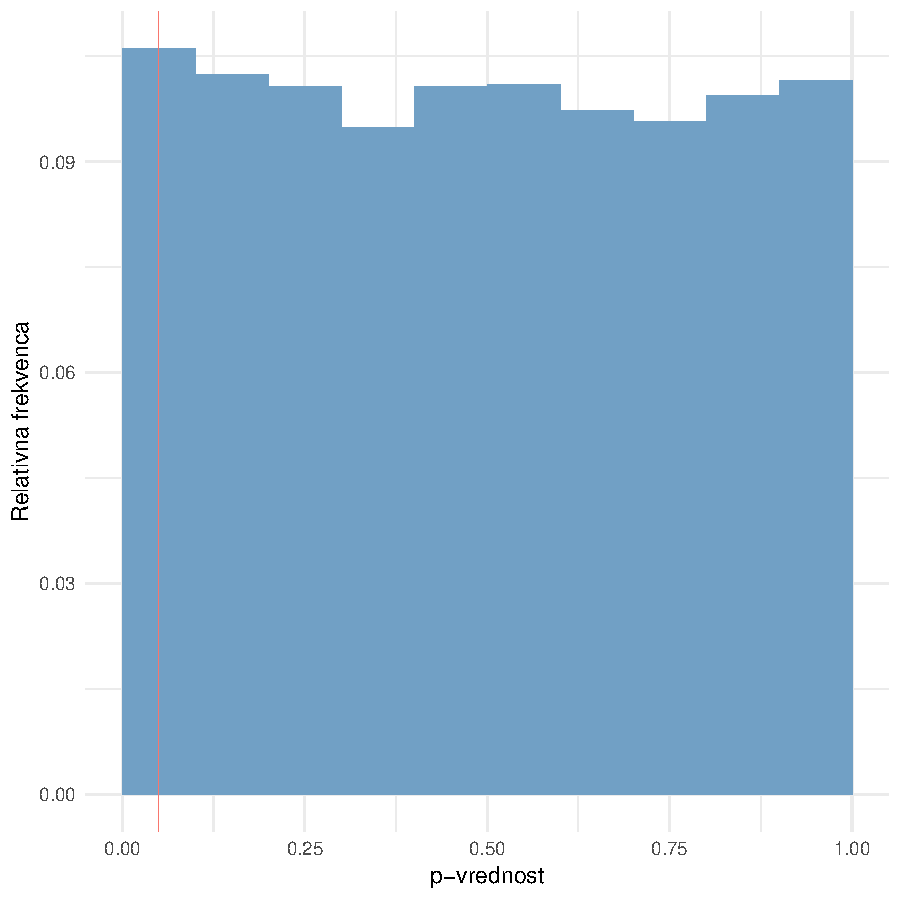
\includegraphics{stadij_H0_M_S1}
    \subcaption{H0}
    \label{fig:1a}
  \end{minipage}%
  \begin{minipage}[b]{.4\linewidth}
    \centering
    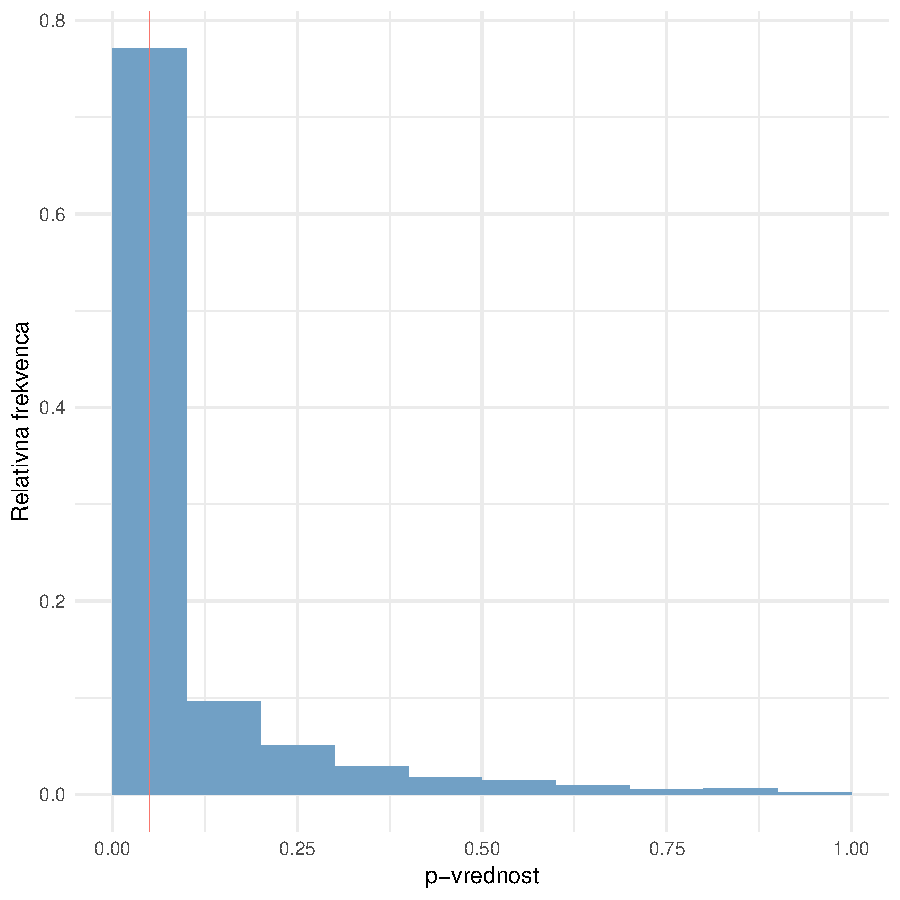
\includegraphics{stadij_HA_M_S1}
    \subcaption{HA}
    \label{fig:1b}
  \end{minipage}
  \caption{Porazdelitve p-vrednosti pridobljenih z LRT glede na hipotezo}
  \label{fig:1}
\end{figure}

% % brejka

\newpage
\subsection{Zaplet}
Pri testiranju z modelom s posameznihm zapletom testiramo ali posamezen zaplet vpliva pri izbiri tipa operacije. Polni model tesitra enako hipotezo, vendar ob upoštevanju drugih zapletov.

V primeru zapletov, ki so neodvisno generirani, vidimo da je težava, ki smo jo izpostavili veliko manj prisotna, oziroma je skladanje z načinom, ko smo upoštevali posamezne zaplete in ko smo upoštevali vse zaplete, veliko večje (85\%).

Ko testiramo hipoteze pod alternativno hipotezo opazimo, da je moč testa, ko upoštevamo vse zaplete večja, kot pri modelih s posameznimi zapleti.

% latex table generated in R 3.5.1 by xtable 1.8-2 package
% Wed Apr 24 19:51:15 2019
\begin{table}[ht]
\centering
\begin{tabular}{rrrrrrrrrrr}
  \hline
 & Z1 & Z2 & Z3 & Z4 & Z5 & Z6 & Z7 & Z8 & Z9 & Z10 \\ 
  \hline
P(zavrneU) & 0.043 & 0.044 & 0.053 & 0.052 & 0.047 & 0.050 & 0.046 & 0.048 & 0.051 & 0.053 \\ 
  P(zavrneM) & 0.047 & 0.049 & 0.055 & 0.056 & 0.050 & 0.054 & 0.051 & 0.051 & 0.054 & 0.053 \\ 
  P(zavrneM $|$ zavrenU) & 0.866 & 0.878 & 0.851 & 0.851 & 0.872 & 0.878 & 0.858 & 0.838 & 0.884 & 0.856 \\ 
  P(zavrneU $|$ zavrenM) & 0.793 & 0.775 & 0.817 & 0.804 & 0.821 & 0.815 & 0.785 & 0.788 & 0.824 & 0.860 \\ 
   \hline
\end{tabular}
\caption{Verjetnosti zavrnitev pri H0} 
\label{table:6}
\end{table}
% latex table generated in R 3.5.1 by xtable 1.8-2 package
% Wed Apr 24 19:51:15 2019
\begin{table}[ht]
\centering
\begin{tabular}{rrrrrrrrrrr}
  \hline
 & Z1 & Z2 & Z3 & Z4 & Z5 & Z6 & Z7 & Z8 & Z9 & Z10 \\ 
  \hline
P(zavrneU) & 0.936 & 0.994 & 0.996 & 0.979 & 0.893 & 0.616 & 0.551 & 0.356 & 0.212 & 0.116 \\ 
  P(zavrneM) & 0.930 & 0.987 & 0.999 & 0.997 & 0.965 & 0.786 & 0.722 & 0.506 & 0.289 & 0.112 \\ 
  P(zavrneM $|$ zavrenU) & 0.993 & 0.992 & 0.999 & 0.999 & 0.991 & 0.956 & 0.942 & 0.881 & 0.746 & 0.557 \\ 
  P(zavrneU $|$ zavrenM) & 0.999 & 0.999 & 0.997 & 0.980 & 0.917 & 0.749 & 0.718 & 0.620 & 0.548 & 0.576 \\ 
   \hline
\end{tabular}
\caption{Verjetnosti zavrnitev pri HA} 
\label{table:7}
\end{table}


%\newpage
%\subsubsection{H0}
%
%\begin{figure}[h]
%  \centering
%  \begin{minipage}[b]{.4\linewidth}
%    \centering
%    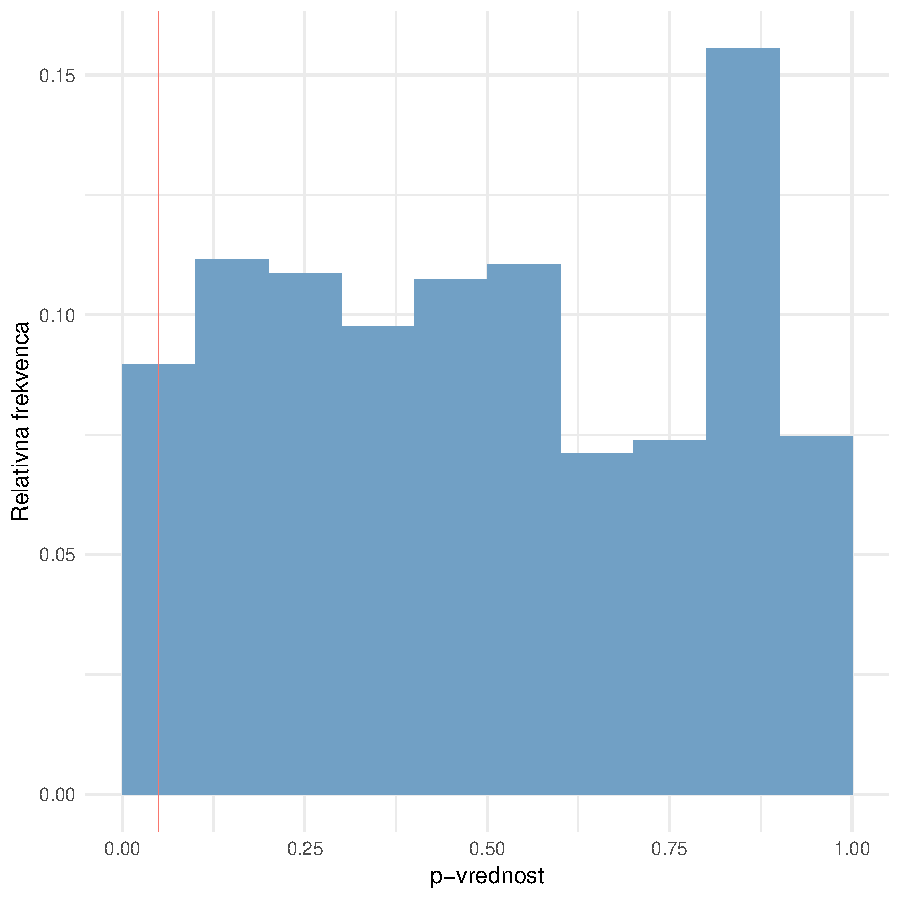
\includegraphics{zaplet_H0_U_Z1}
%    \subcaption{Zaplet 1 (beta = 0) - U}
%    \label{fig:1b}
%  \end{minipage}
%  \begin{minipage}[b]{.4\linewidth}
%    \centering
%    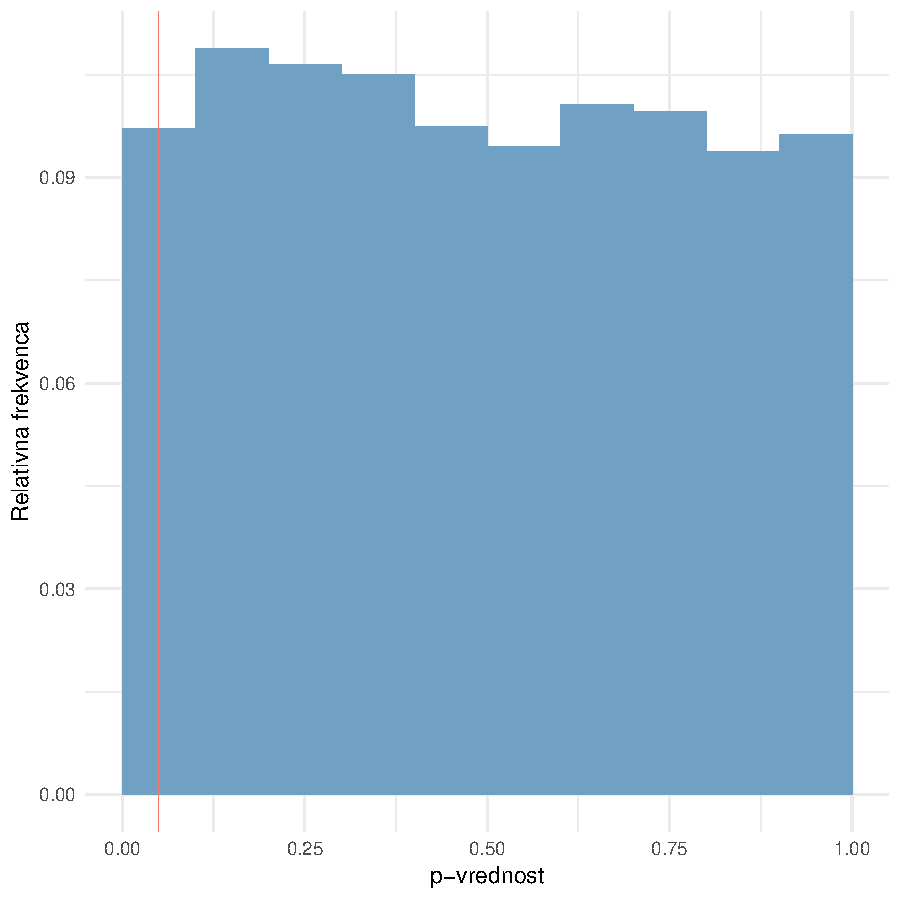
\includegraphics{zaplet_H0_M_Z1}
%    \subcaption{Zaplet 1 (beta = 0) - M}
%    \label{fig:1b}
%  \end{minipage}
%  \begin{minipage}[b]{.4\linewidth}
%    \centering
%    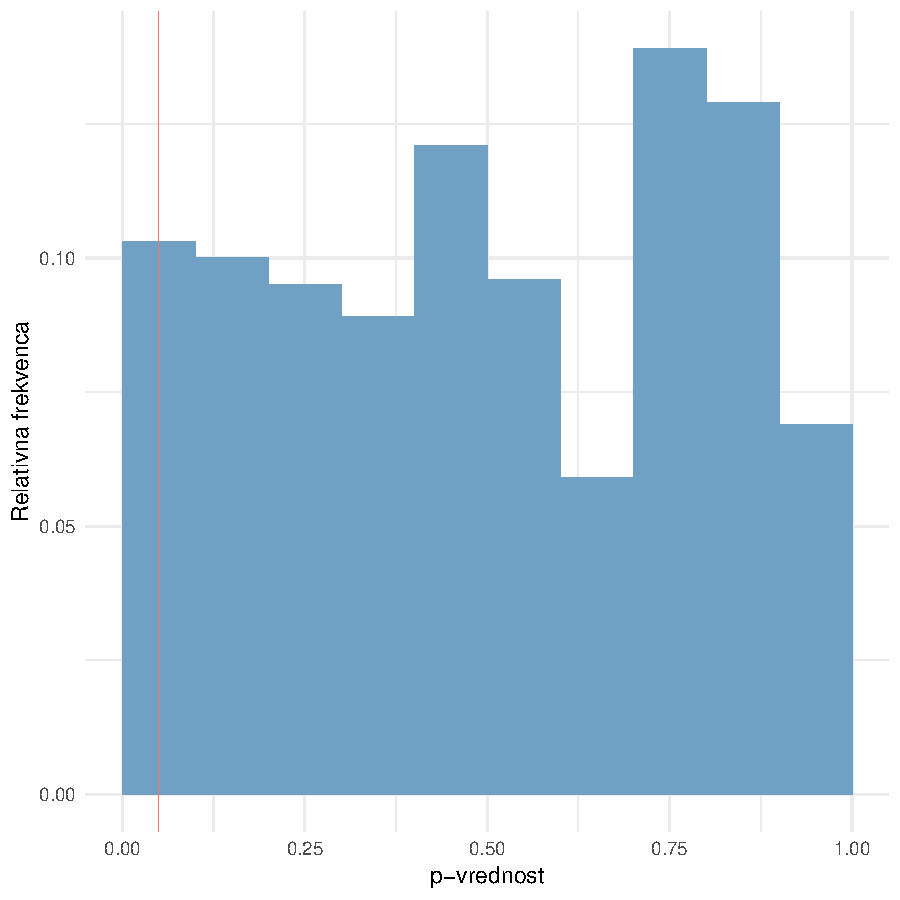
\includegraphics{zaplet_H0_U_Z2}
%    \subcaption{Zaplet 2 (beta = 0) - U}
%    \label{fig:1b}
%  \end{minipage}
%  \begin{minipage}[b]{.4\linewidth}
%    \centering
%    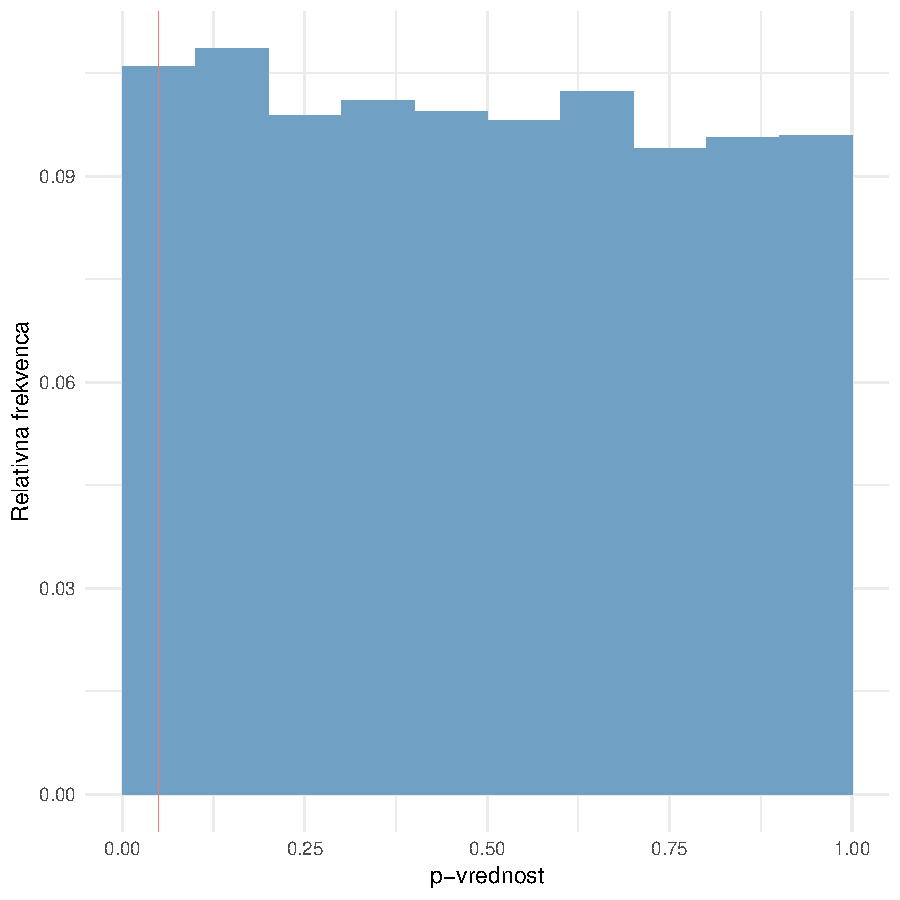
\includegraphics{zaplet_H0_M_Z2}
%    \subcaption{Zaplet 2 (beta = 0) - M}
%    \label{fig:1b}
%  \end{minipage}
%  \caption{Porazdelitve p-vrednosti pri H0 gleda na zaplet in model (1/3)}
%  \label{fig:1}
%\end{figure}
%
%\clearpage
%\newpage
%\begin{figure}[t]
%  \centering
%  \begin{minipage}[b]{.4\linewidth}
%    \centering
%    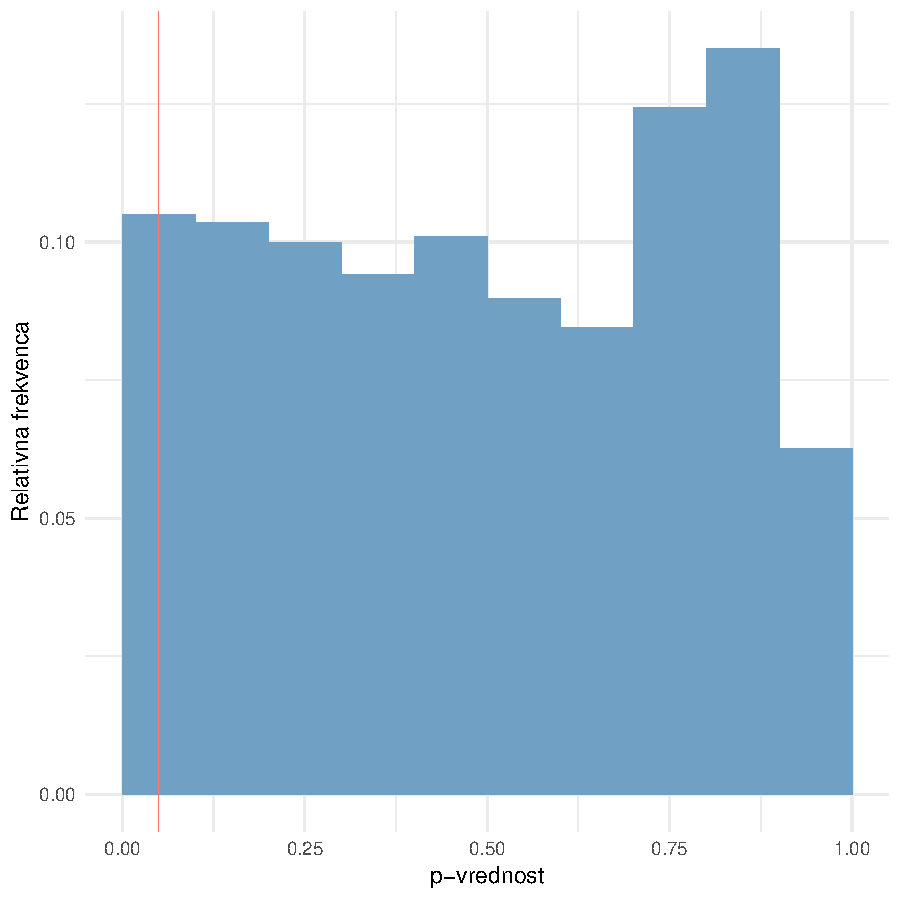
\includegraphics{zaplet_H0_U_Z3}
%    \subcaption{Zaplet 3 (beta = 0) - U}
%    \label{fig:1b}
%  \end{minipage}
%  \begin{minipage}[b]{.4\linewidth}
%    \centering
%    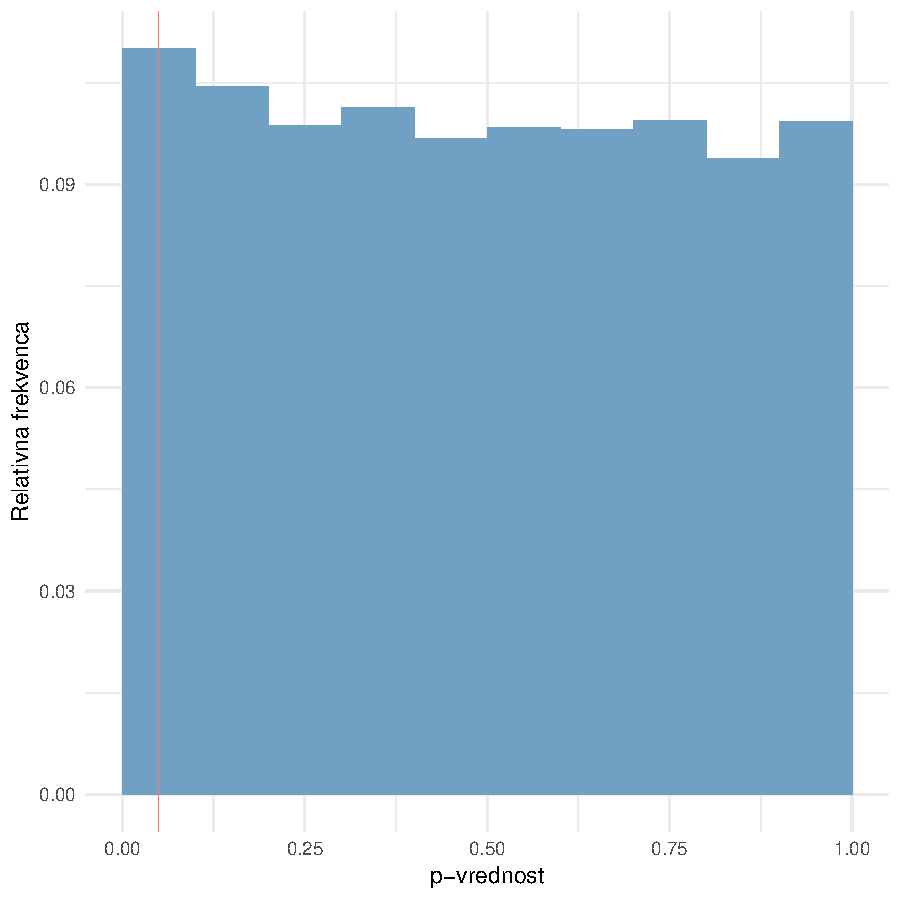
\includegraphics{zaplet_H0_M_Z3}
%    \subcaption{Zaplet 3 (beta = 0) - M}
%    \label{fig:1b}
%  \end{minipage}
%    \begin{minipage}[b]{.4\linewidth}
%    \centering
%    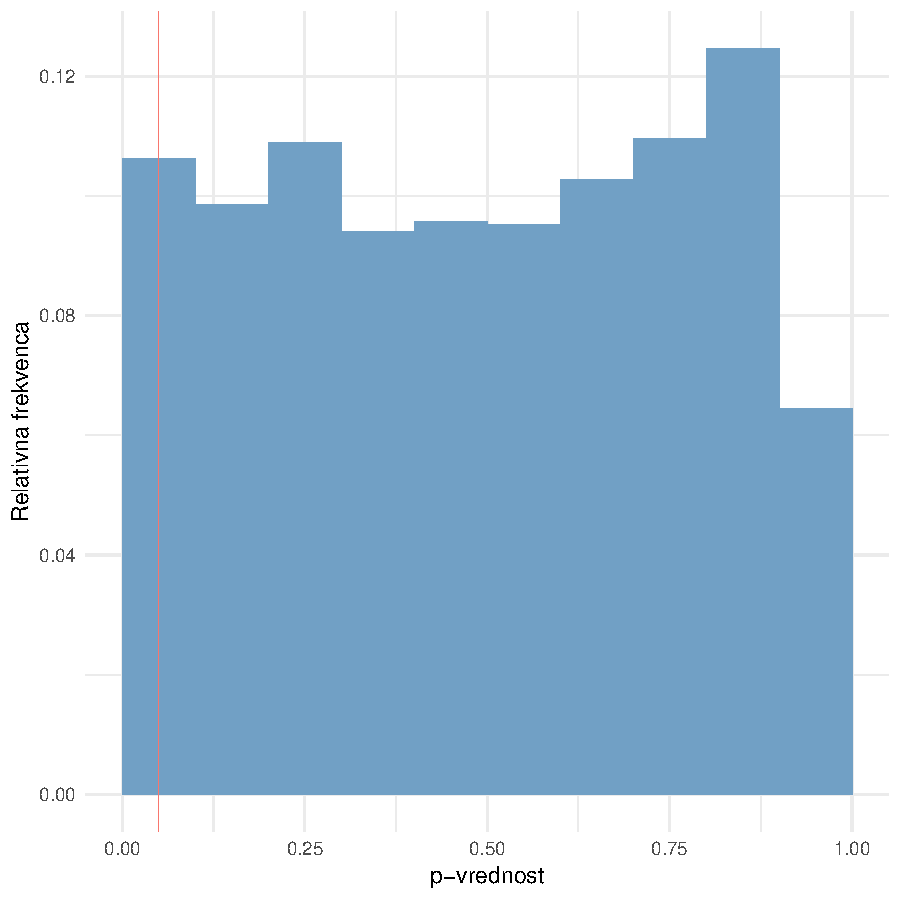
\includegraphics{zaplet_H0_U_Z4}
%    \subcaption{Zaplet 4 (beta = 0) - U}
%    \label{fig:1b}
%  \end{minipage}
%  \begin{minipage}[b]{.4\linewidth}
%    \centering
%    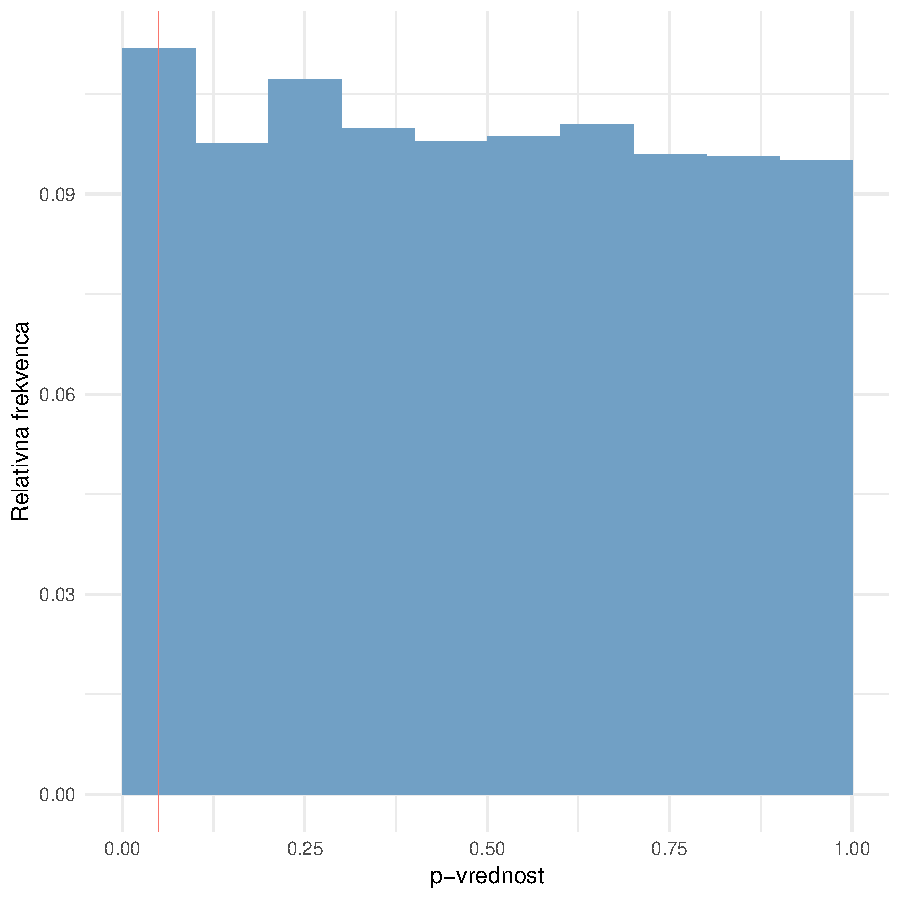
\includegraphics{zaplet_H0_M_Z4}
%    \subcaption{Zaplet 4 (beta = 0) - M}
%    \label{fig:1b}
%  \end{minipage}
%  \begin{minipage}[b]{.4\linewidth}
%    \centering
%    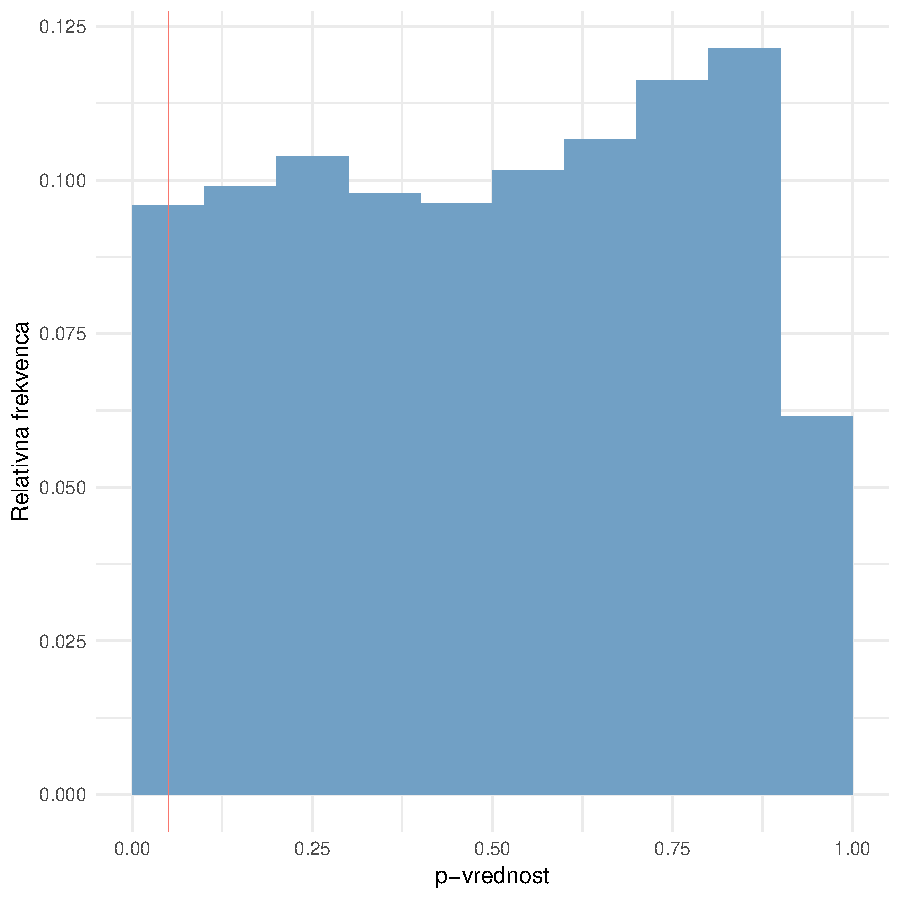
\includegraphics{zaplet_H0_U_Z5}
%    \subcaption{Zaplet 5 (beta = 0) - U}
%    \label{fig:1b}
%  \end{minipage}
%  \begin{minipage}[b]{.4\linewidth}
%    \centering
%    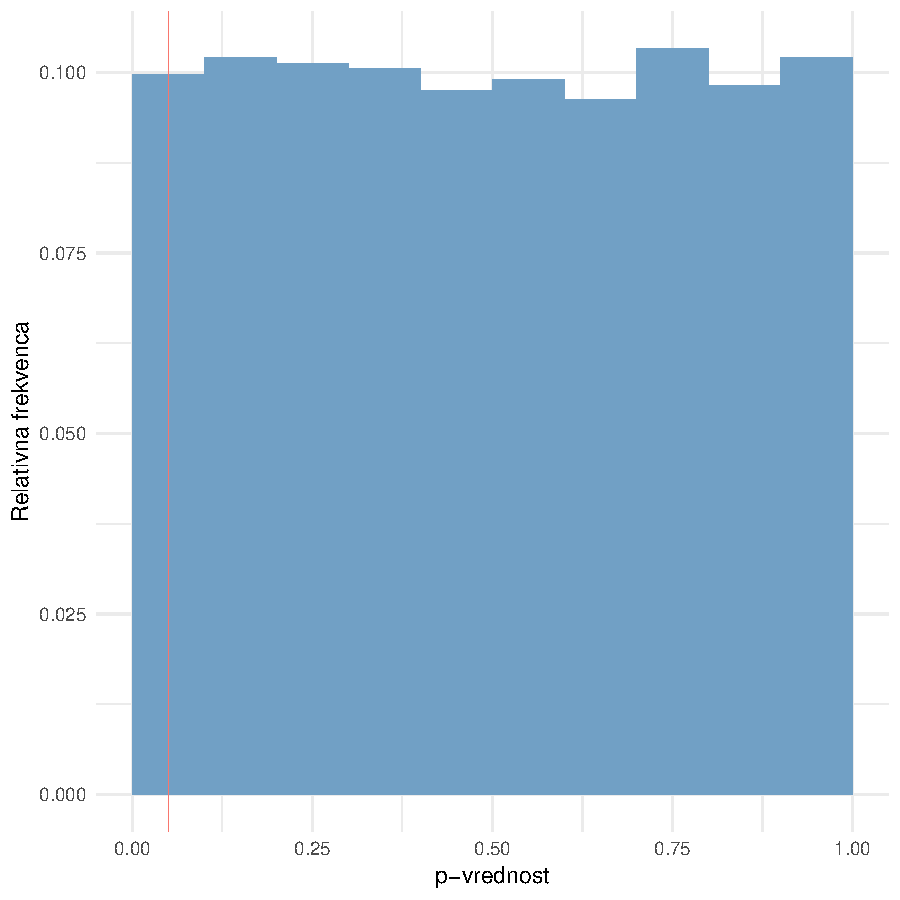
\includegraphics{zaplet_H0_M_Z5}
%    \subcaption{Zaplet 5 (beta = 0) - M}
%    \label{fig:1b}
%  \end{minipage}
%    \begin{minipage}[b]{.4\linewidth}
%    \centering
%    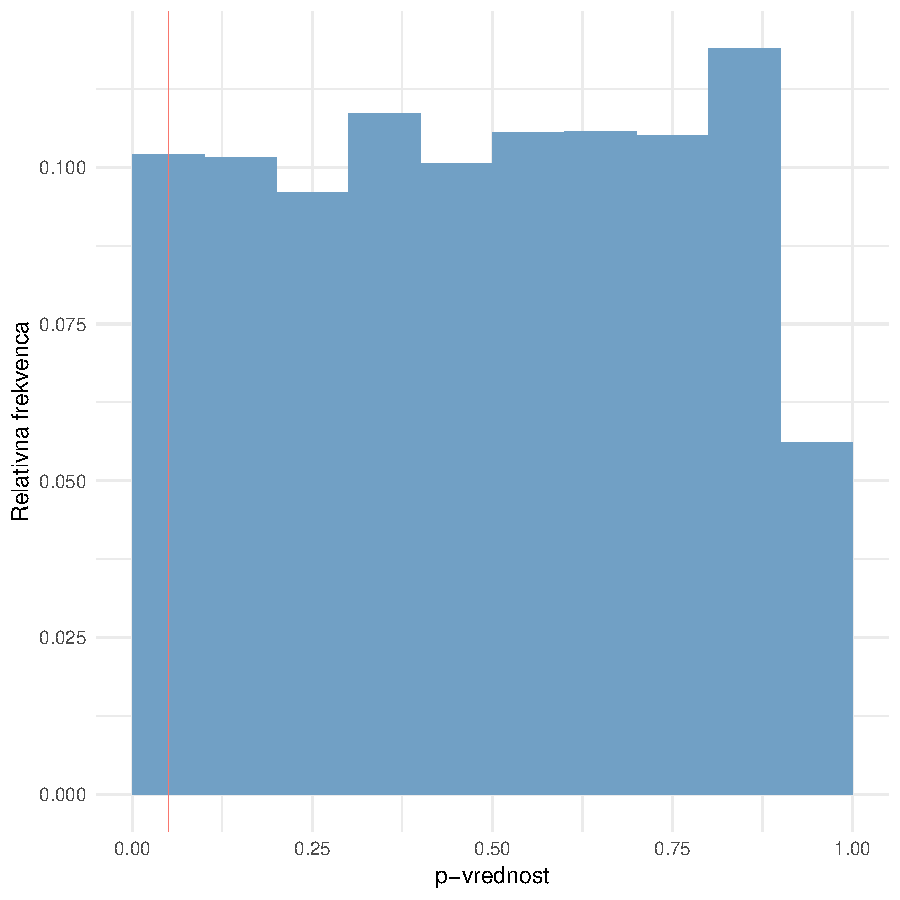
\includegraphics{zaplet_H0_U_Z6}
%    \subcaption{Zaplet 6 (beta = 0) - U}
%    \label{fig:1b}
%  \end{minipage}
%  \begin{minipage}[b]{.4\linewidth}
%    \centering
%    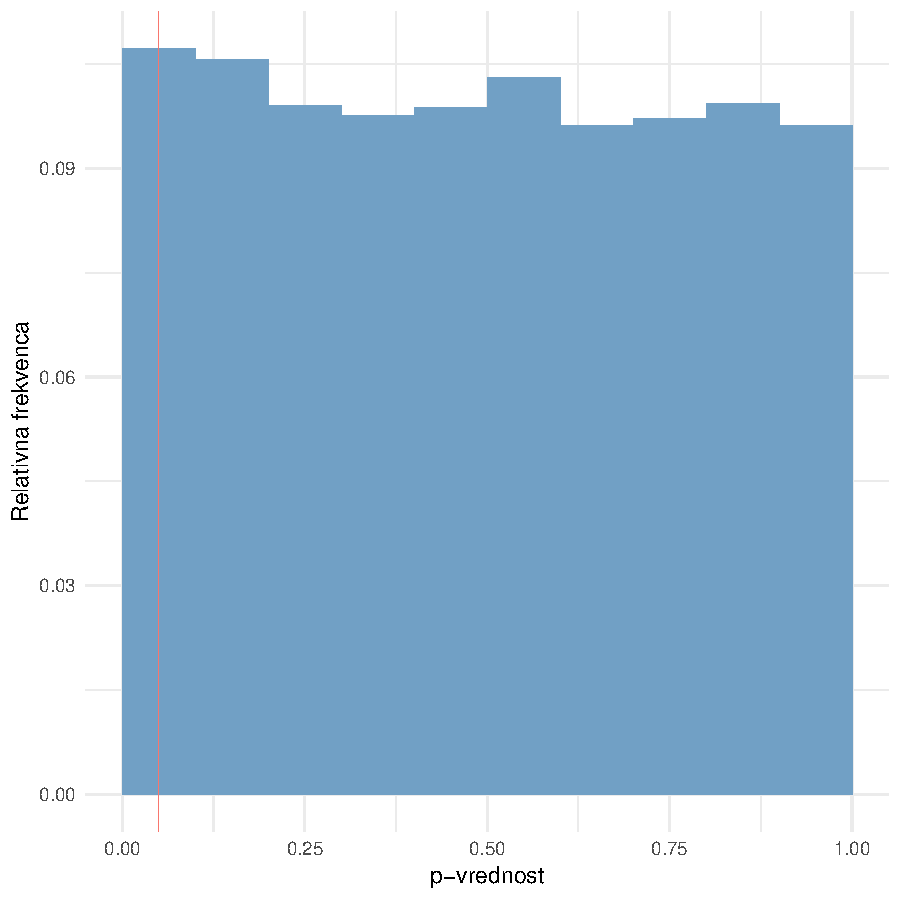
\includegraphics{zaplet_H0_M_Z6}
%    \subcaption{Zaplet 6 (beta = 0) - M}
%    \label{fig:1b}
%  \end{minipage}
%  \caption{Porazdelitve p-vrednosti pri H0 gleda na zaplet in model (2/3)}
%  \label{fig:1}
%\end{figure}
%
%\clearpage
%\newpage
%\begin{figure}[h]
%  \centering
%  \begin{minipage}[b]{.4\linewidth}
%    \centering
%    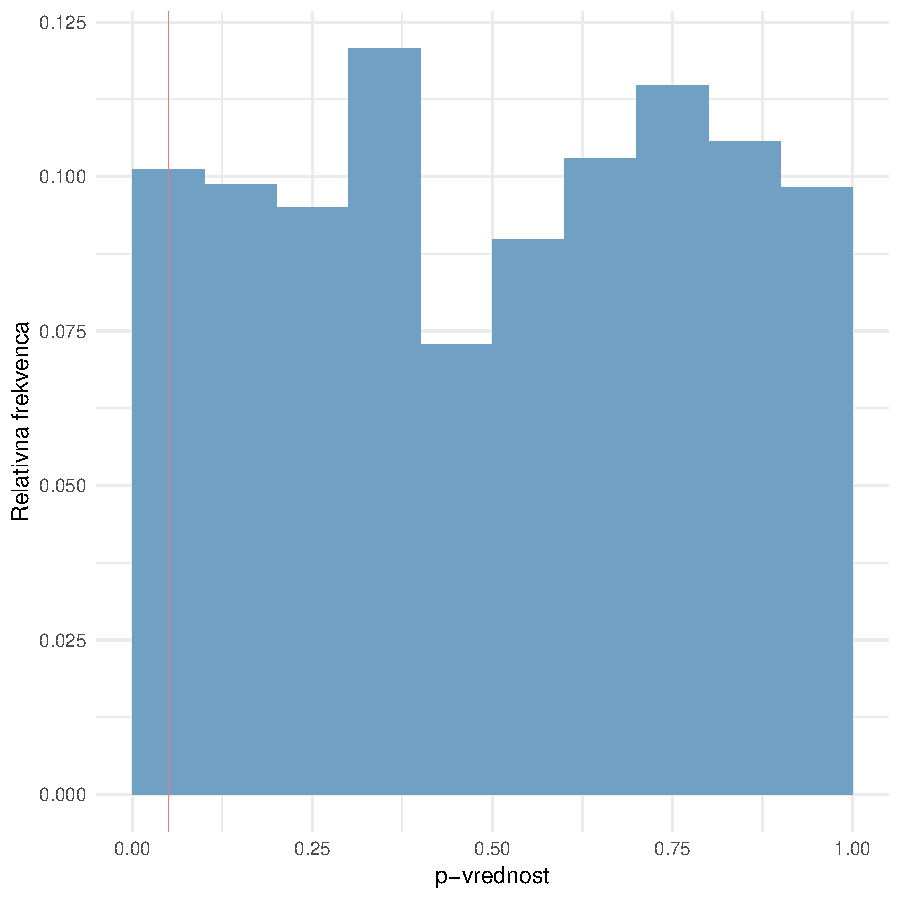
\includegraphics{zaplet_H0_U_Z7}
%    \subcaption{Zaplet 7 (beta = 0) - U}
%    \label{fig:1b}
%  \end{minipage}
%  \begin{minipage}[b]{.4\linewidth}
%    \centering
%    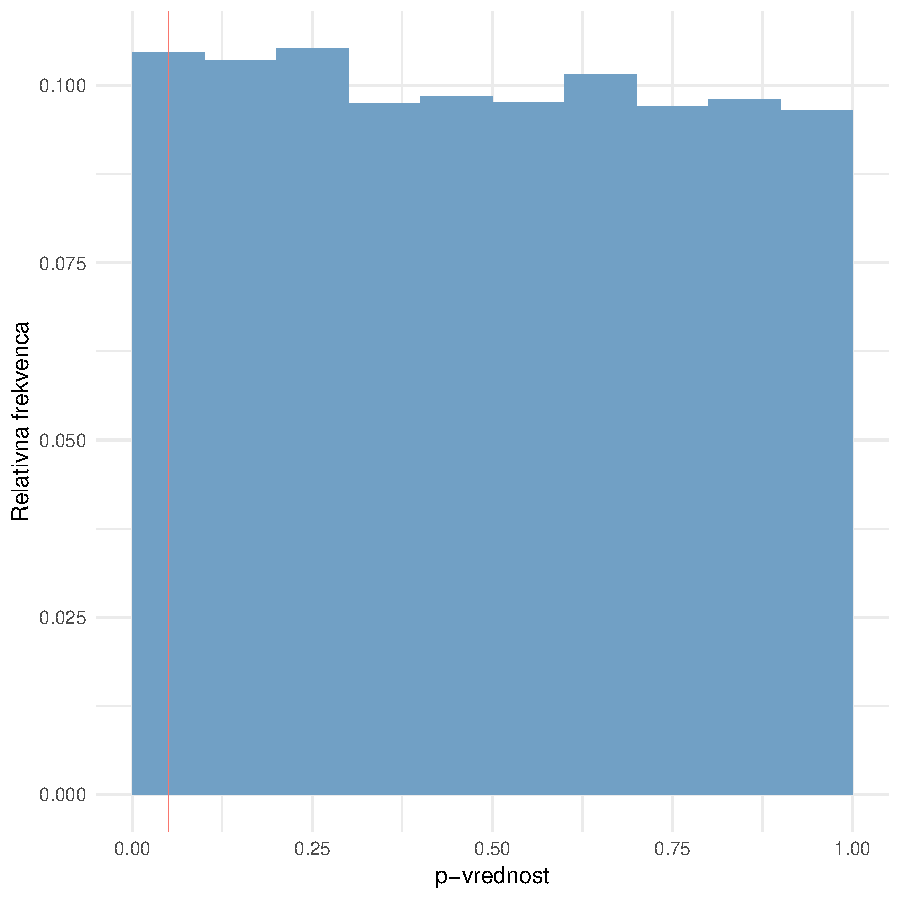
\includegraphics{zaplet_H0_M_Z7}
%    \subcaption{Zaplet 7 (beta = 0) - M}
%    \label{fig:1b}
%  \end{minipage}
%  \begin{minipage}[b]{.4\linewidth}
%    \centering
%    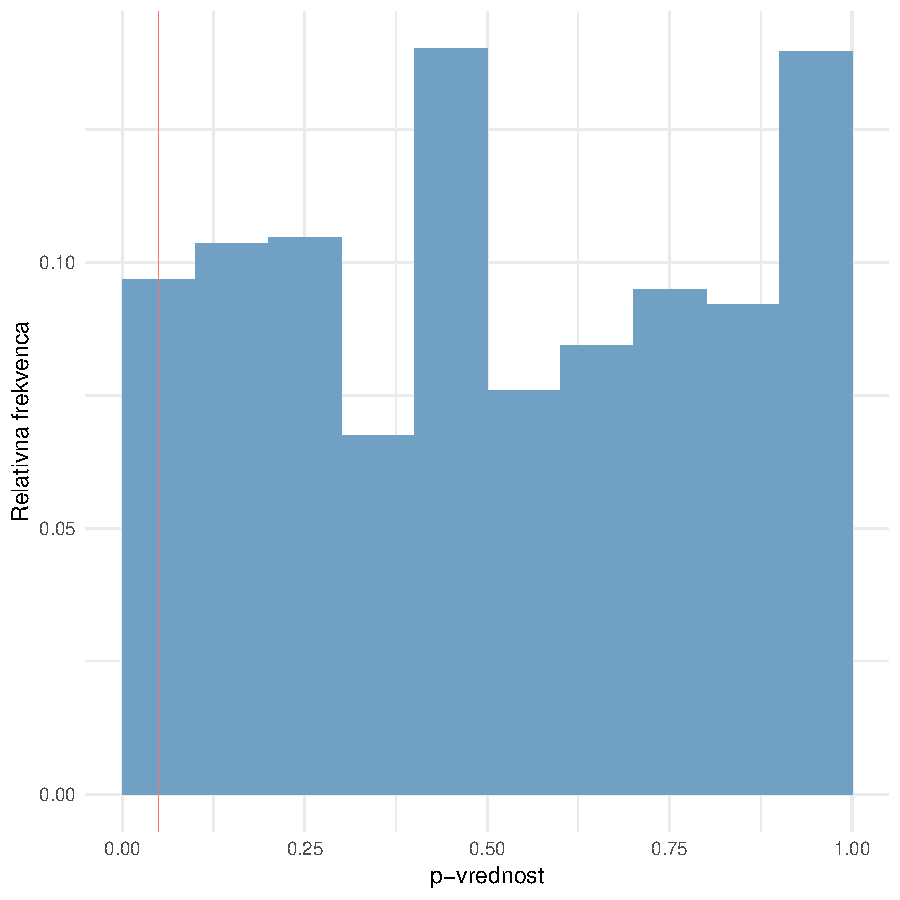
\includegraphics{zaplet_H0_U_Z8}
%    \subcaption{Zaplet 8 (beta = 0) - U}
%    \label{fig:1b}
%  \end{minipage}
%  \begin{minipage}[b]{.4\linewidth}
%    \centering
%    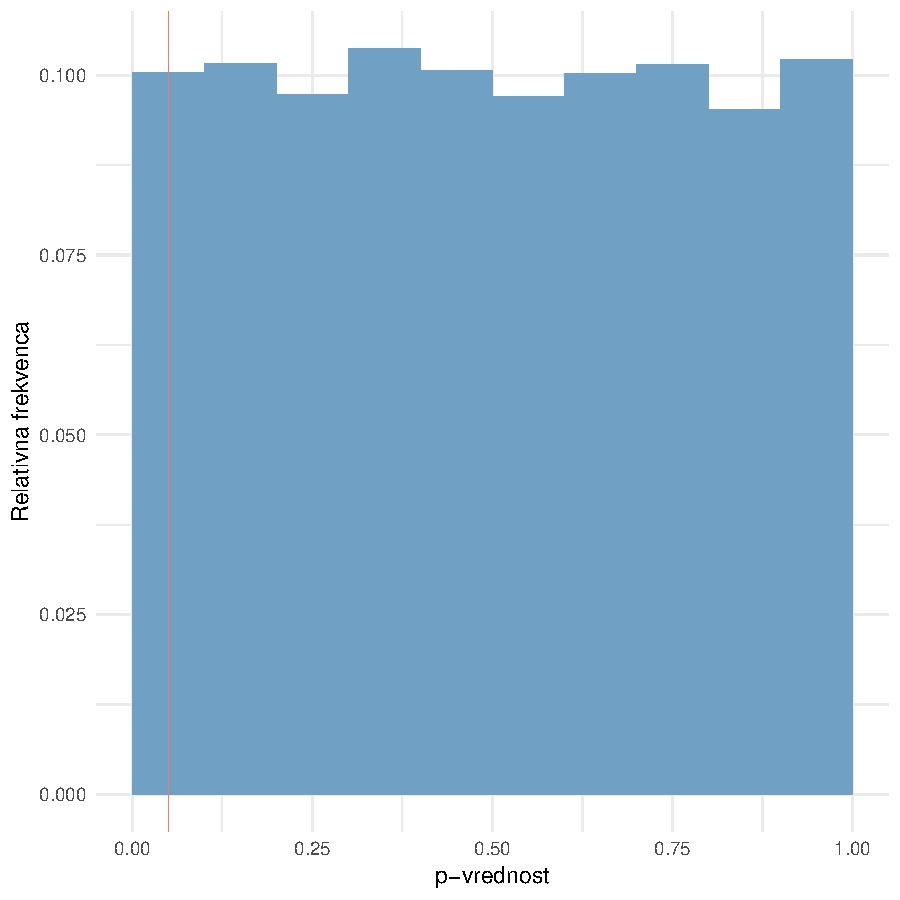
\includegraphics{zaplet_H0_M_Z8}
%    \subcaption{Zaplet 8 (beta = 0) - M}
%    \label{fig:1b}
%  \end{minipage}
%  \begin{minipage}[b]{.4\linewidth}
%    \centering
%    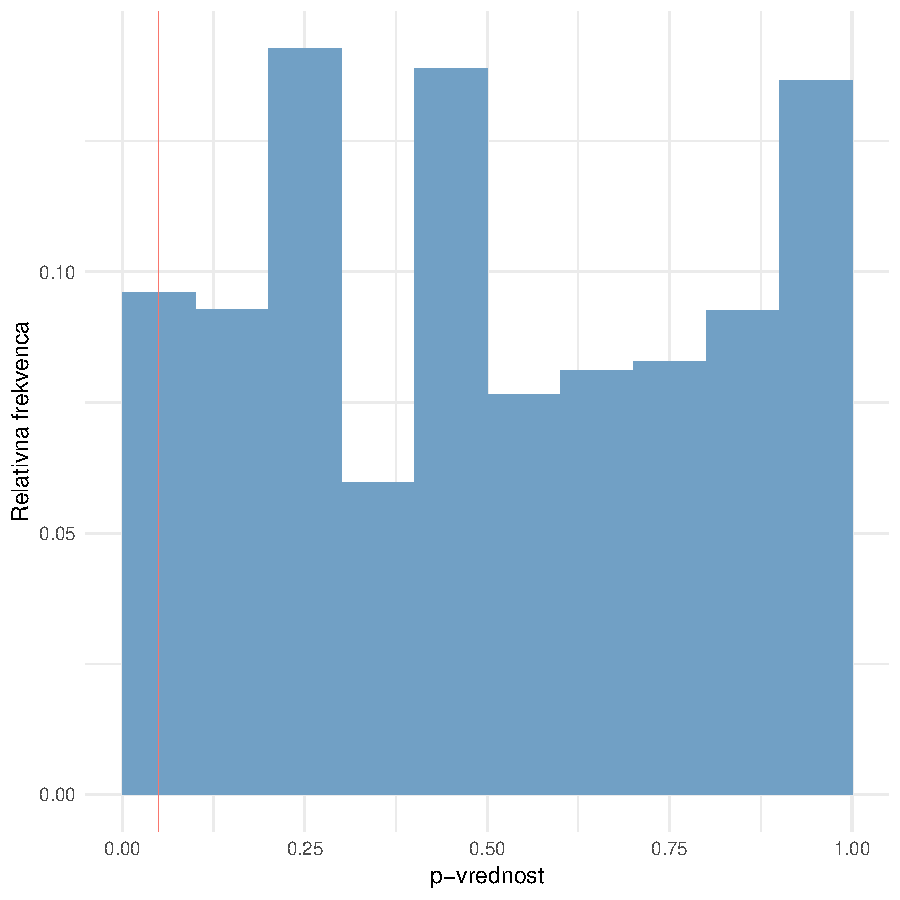
\includegraphics{zaplet_H0_U_Z9}
%    \subcaption{Zaplet 9 (beta = 0) - U}
%    \label{fig:1b}
%  \end{minipage}
%  \begin{minipage}[b]{.4\linewidth}
%    \centering
%    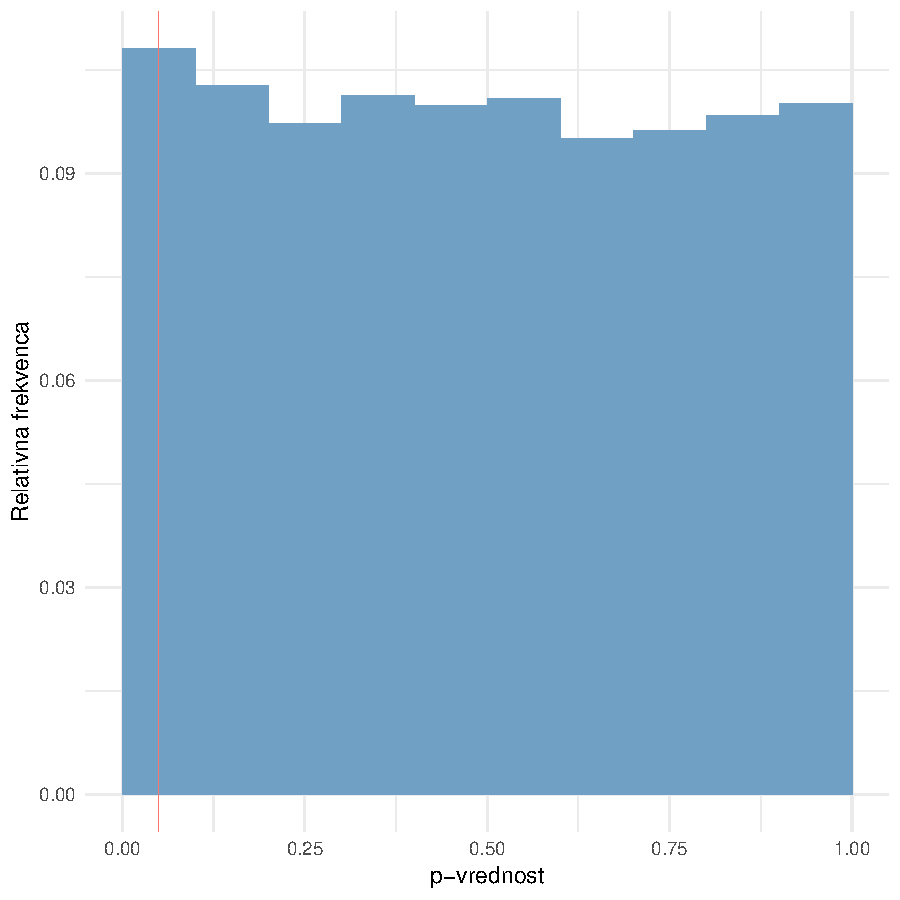
\includegraphics{zaplet_H0_M_Z9}
%    \subcaption{Zaplet 9 (beta = 0) - M}
%    \label{fig:1b}
%  \end{minipage}
%  \begin{minipage}[b]{.4\linewidth}
%    \centering
%    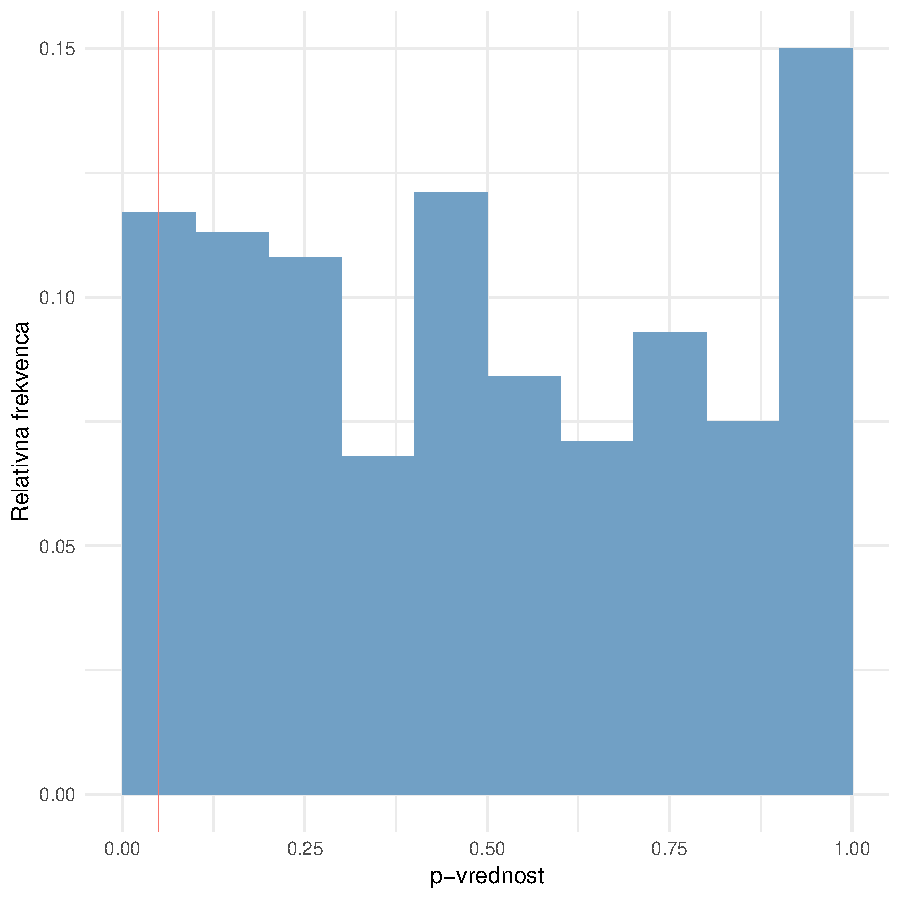
\includegraphics{zaplet_H0_U_Z10}
%    \subcaption{Zaplet 10 (beta = 0) - U}
%    \label{fig:1b}
%  \end{minipage}
%  \begin{minipage}[b]{.4\linewidth}
%    \centering
%    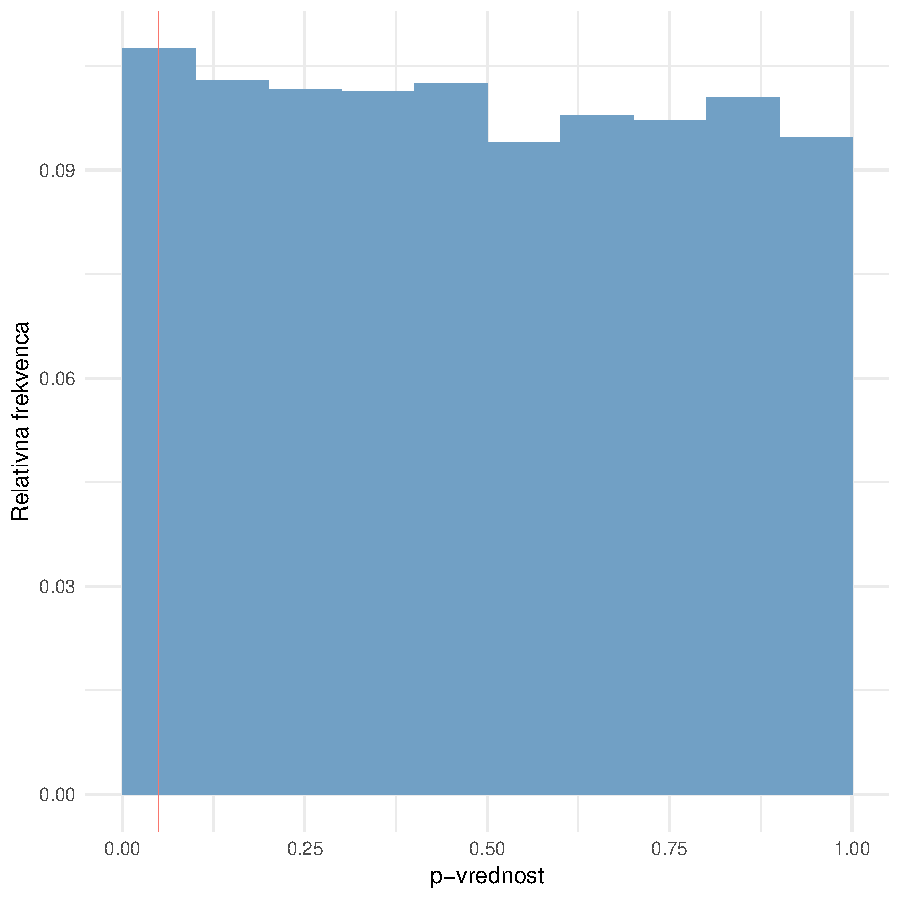
\includegraphics{zaplet_H0_M_Z10}
%    \subcaption{Zaplet 10 (beta = 0) - M}
%    \label{fig:1b}
%  \end{minipage}
%  \caption{Porazdelitve p-vrednosti pri H0 gleda na zaplet in model (3/3)}
%  \label{fig:1}
%\end{figure}
%
%\clearpage
%\newpage
%\subsubsection{HA}
%
%\begin{figure}[h]
%  \centering
%  \begin{minipage}[b]{.4\linewidth}
%    \centering
%    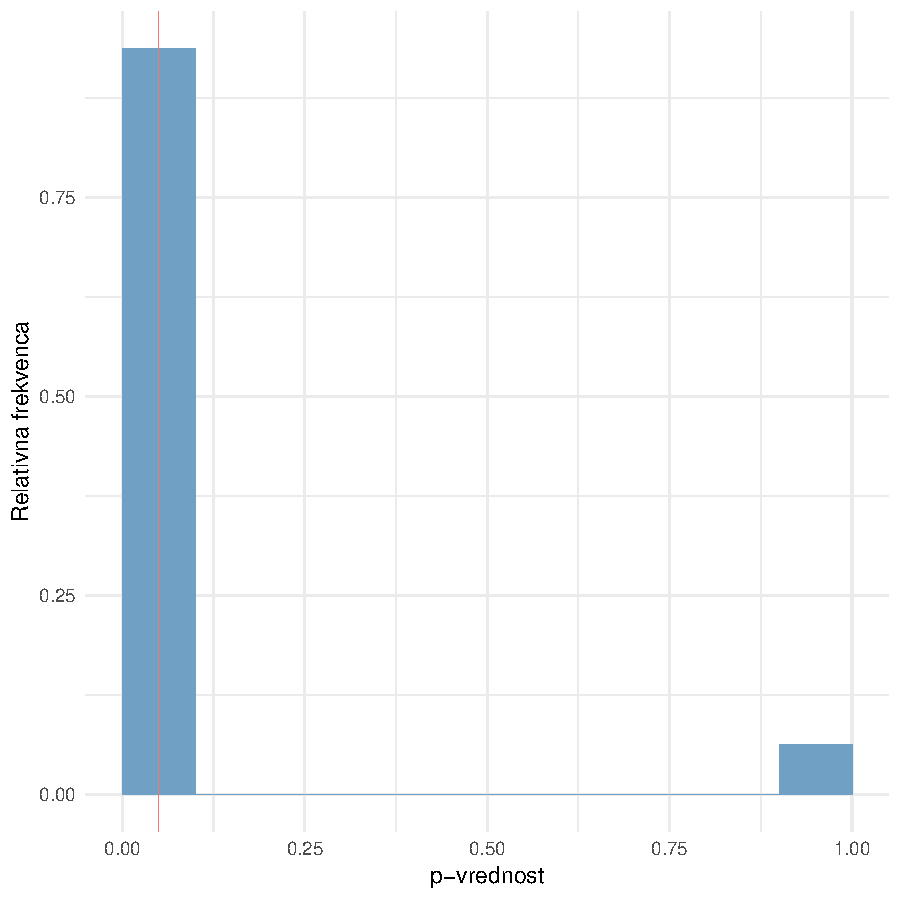
\includegraphics{zaplet_HA_U_Z1}
%    \subcaption{Zaplet 1 (beta = -3.5) - U}
%    \label{fig:1b}
%  \end{minipage}
%  \begin{minipage}[b]{.4\linewidth}
%    \centering
%    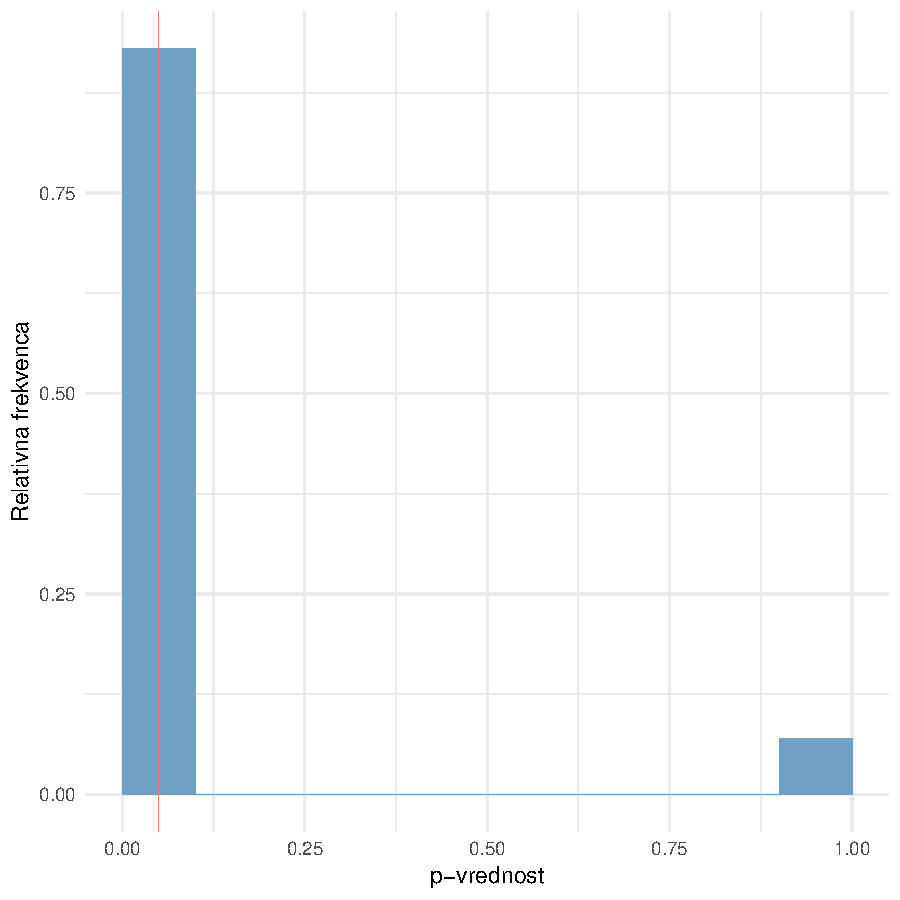
\includegraphics{zaplet_HA_M_Z1}
%    \subcaption{Zaplet 1 (beta = -3.5) - M}
%    \label{fig:1b}
%  \end{minipage}
%  \begin{minipage}[b]{.4\linewidth}
%    \centering
%    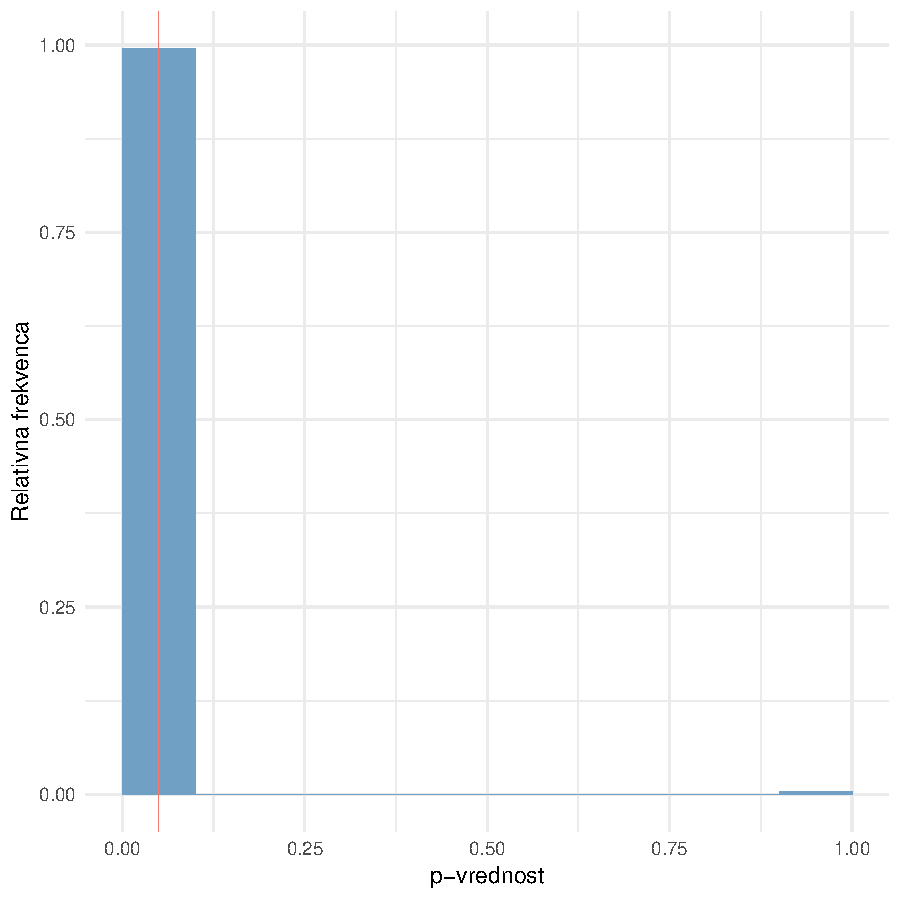
\includegraphics{zaplet_HA_U_Z2}
%    \subcaption{Zaplet 2 (beta = 3) - U}
%    \label{fig:1b}
%  \end{minipage}
%  \begin{minipage}[b]{.4\linewidth}
%    \centering
%    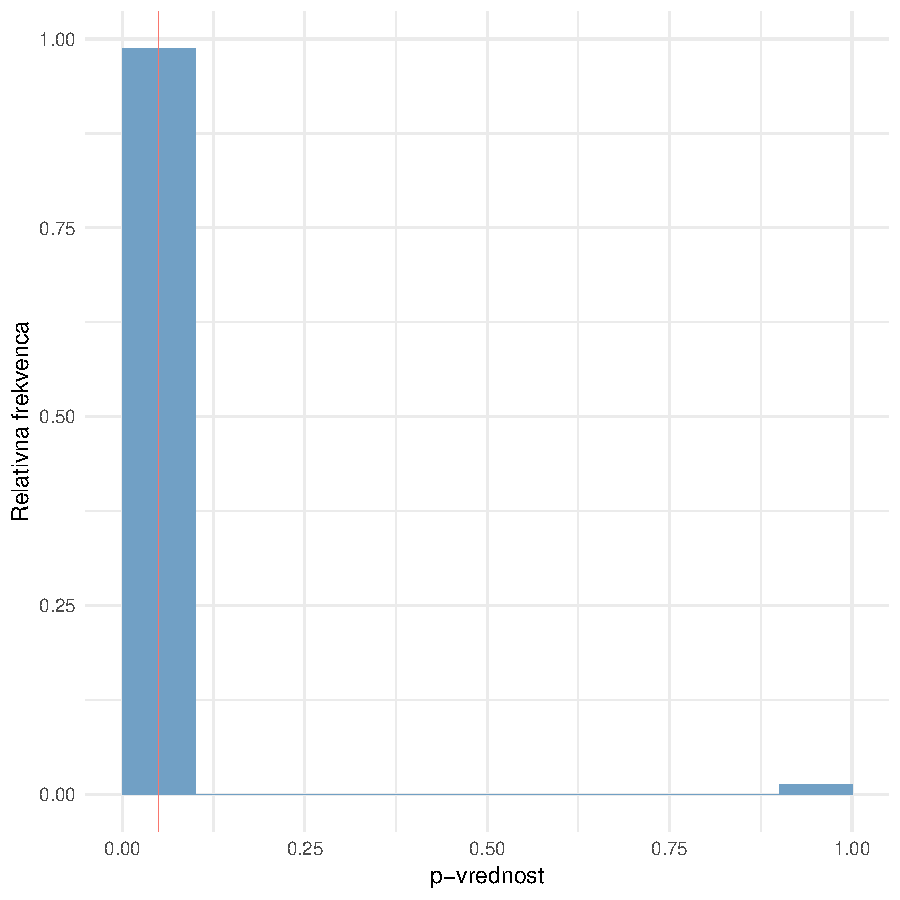
\includegraphics{zaplet_HA_M_Z2}
%    \subcaption{Zaplet 2 (beta = 3) - M}
%    \label{fig:1b}
%  \end{minipage}
%  \caption{Porazdelitve p-vrednosti pri HA gleda na zaplet in model (1/3)}
%  \label{fig:1}
%\end{figure}
%
%\clearpage
%\newpage
%\begin{figure}[h]
%  \centering
%  \begin{minipage}[b]{.4\linewidth}
%    \centering
%    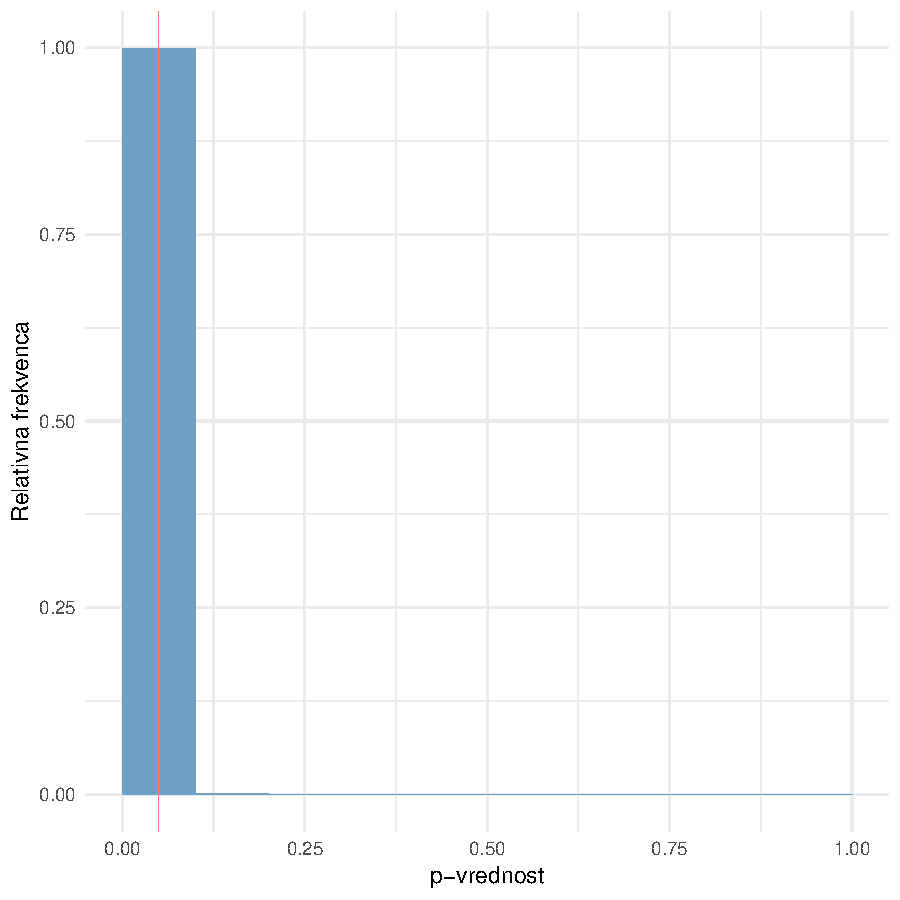
\includegraphics{zaplet_HA_U_Z3}
%    \subcaption{Zaplet 3 (beta = -2.5) - U}
%    \label{fig:1b}
%  \end{minipage}
%  \begin{minipage}[b]{.4\linewidth}
%    \centering
%    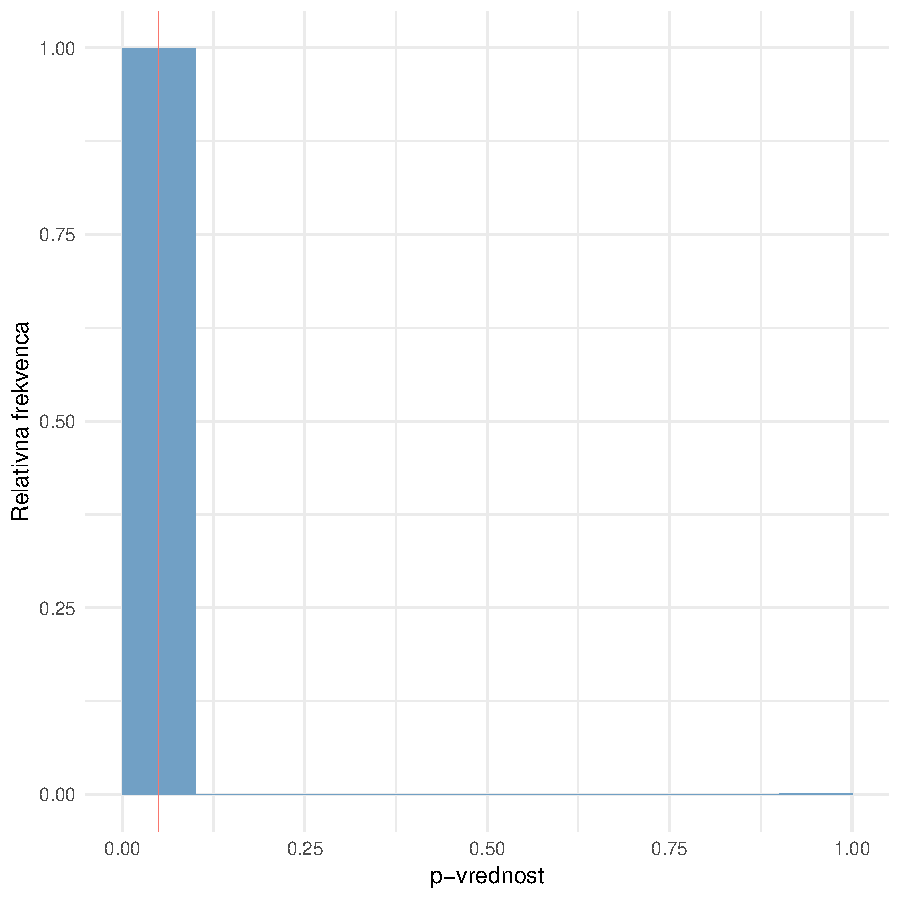
\includegraphics{zaplet_HA_M_Z3}
%    \subcaption{Zaplet 3 (beta = -2.5) - M}
%    \label{fig:1b}
%  \end{minipage}
%    \begin{minipage}[b]{.4\linewidth}
%    \centering
%    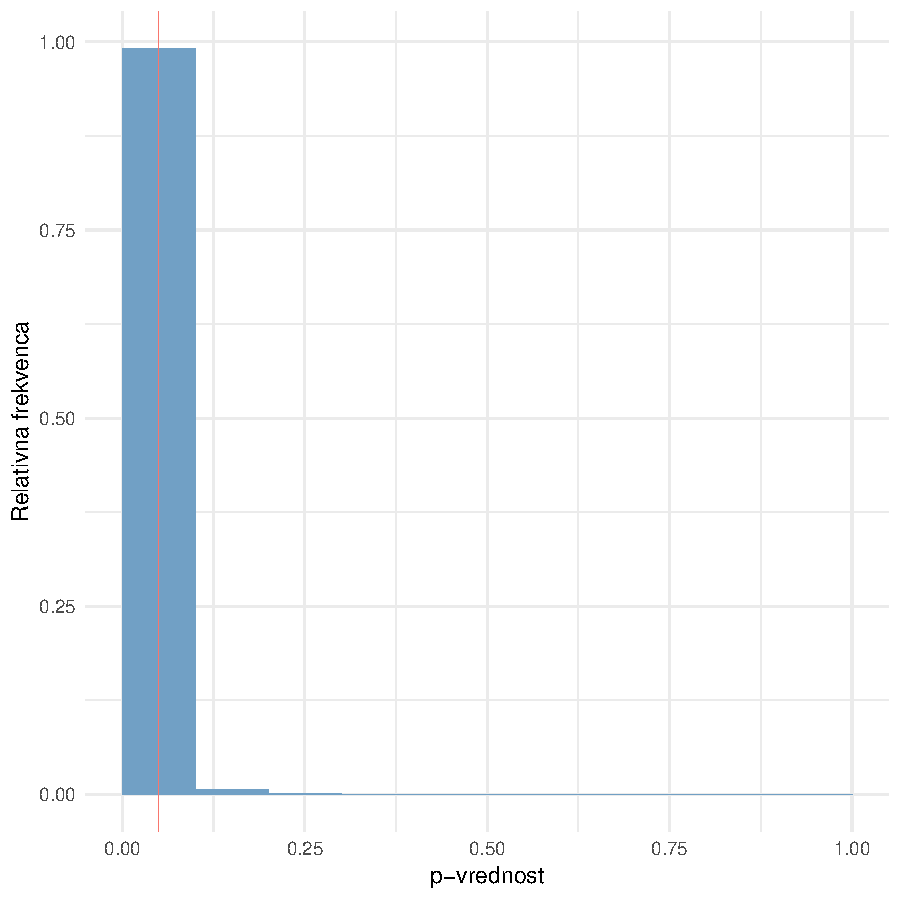
\includegraphics{zaplet_HA_U_Z4}
%    \subcaption{Zaplet 4 (beta = 2) - U}
%    \label{fig:1b}
%  \end{minipage}
%  \begin{minipage}[b]{.4\linewidth}
%    \centering
%    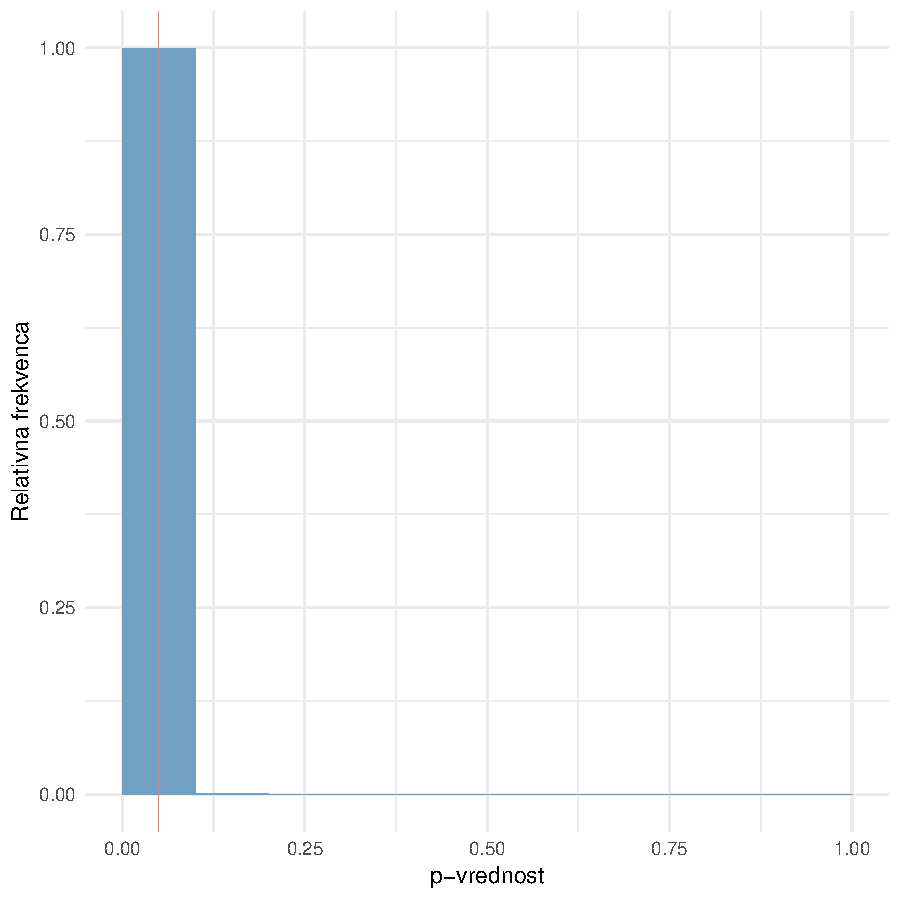
\includegraphics{zaplet_HA_M_Z4}
%    \subcaption{Zaplet 4 (beta = 2) - M}
%    \label{fig:1b}
%  \end{minipage}
%  \begin{minipage}[b]{.4\linewidth}
%    \centering
%    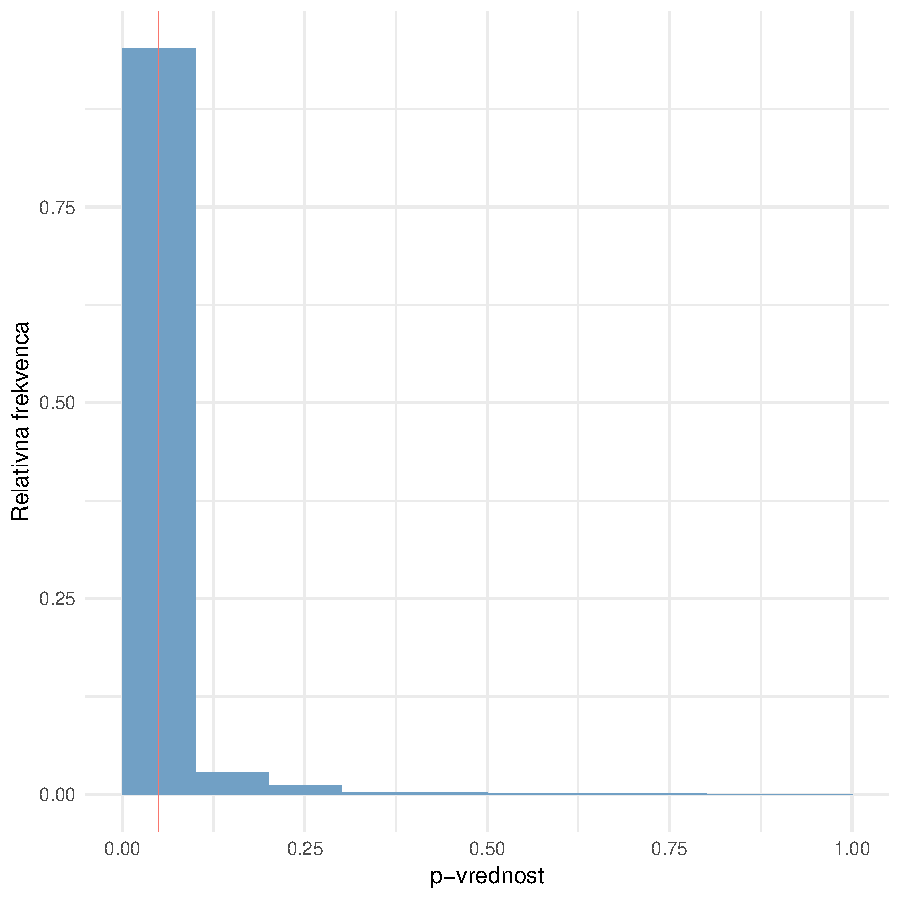
\includegraphics{zaplet_HA_U_Z5}
%    \subcaption{Zaplet 5 (beta = -1.5) - U}
%    \label{fig:1b}
%  \end{minipage}
%  \begin{minipage}[b]{.4\linewidth}
%    \centering
%    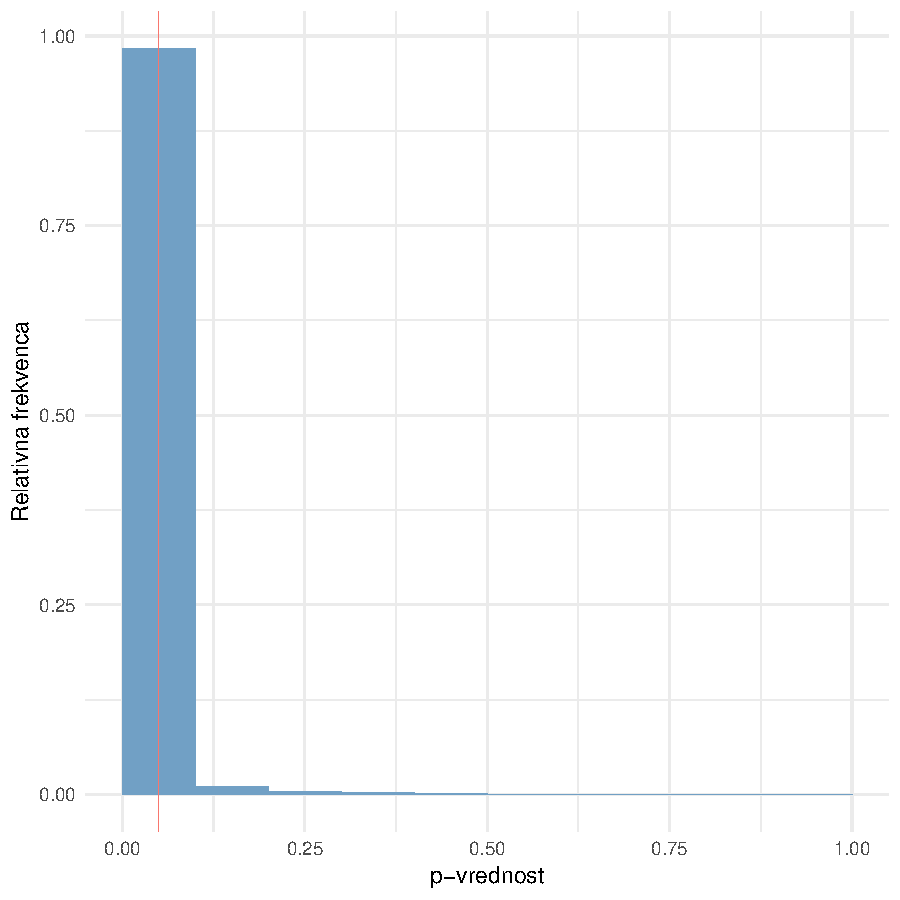
\includegraphics{zaplet_HA_M_Z5}
%    \subcaption{Zaplet 5 (beta = -1.5) - M}
%    \label{fig:1b}
%  \end{minipage}
%    \begin{minipage}[b]{.4\linewidth}
%    \centering
%    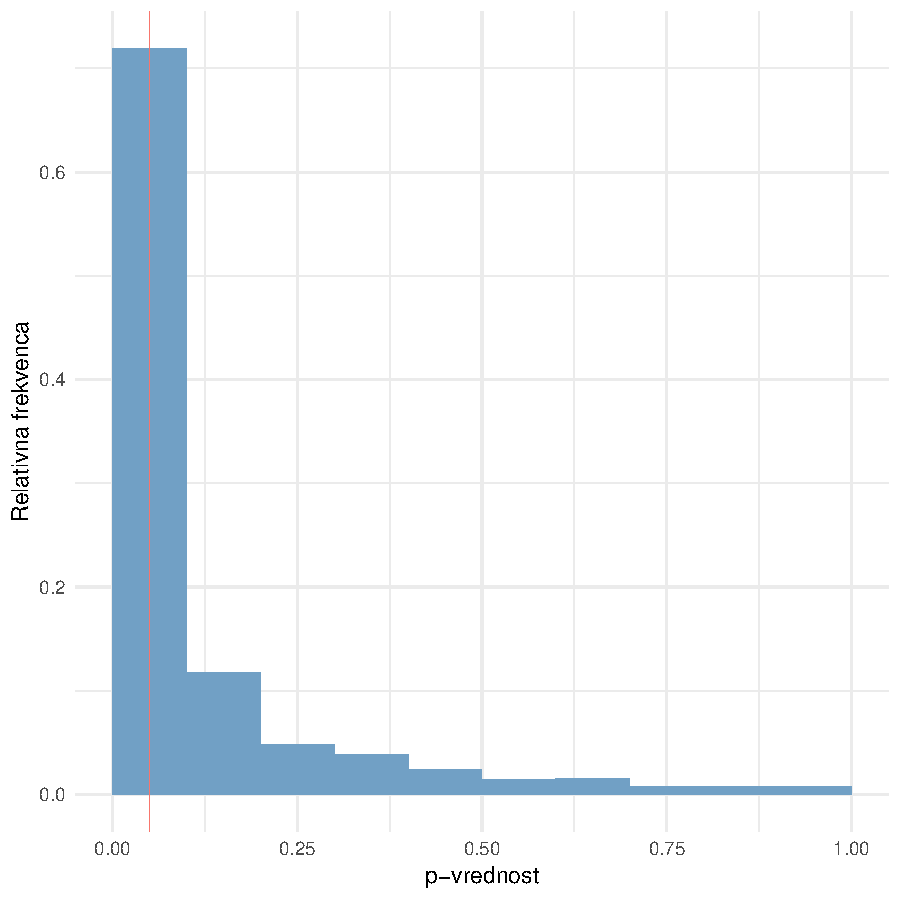
\includegraphics{zaplet_HA_U_Z6}
%    \subcaption{Zaplet 6 (beta = 1) - U}
%    \label{fig:1b}
%  \end{minipage}
%  \begin{minipage}[b]{.4\linewidth}
%    \centering
%    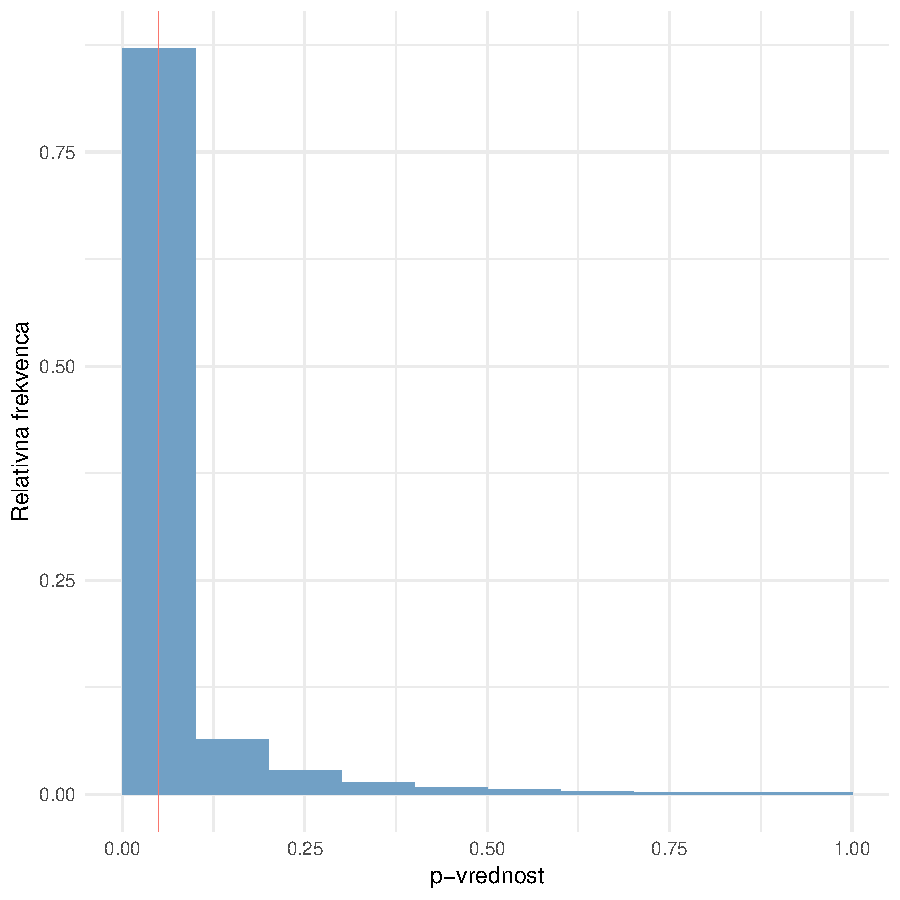
\includegraphics{zaplet_HA_M_Z6}
%    \subcaption{Zaplet 6 (beta = 1) - M}
%    \label{fig:1b}
%  \end{minipage}
%  \caption{Porazdelitve p-vrednosti pri HA gleda na zaplet in model (2/3)}
%  \label{fig:1}
%\end{figure}
%
%\clearpage
%\newpage
%\begin{figure}[h]
%  \centering
%  \begin{minipage}[b]{.4\linewidth}
%    \centering
%    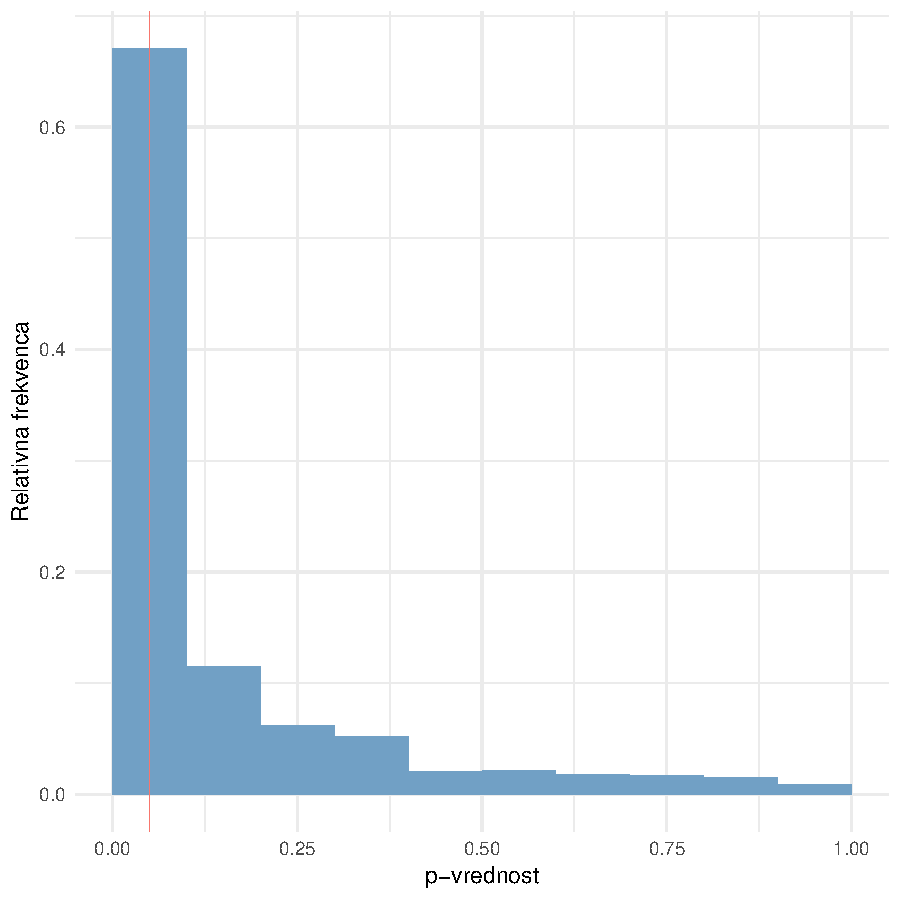
\includegraphics{zaplet_HA_U_Z7}
%    \subcaption{Zaplet 7 (beta = -0.8) - U}
%    \label{fig:1b}
%  \end{minipage}
%  \begin{minipage}[b]{.4\linewidth}
%    \centering
%    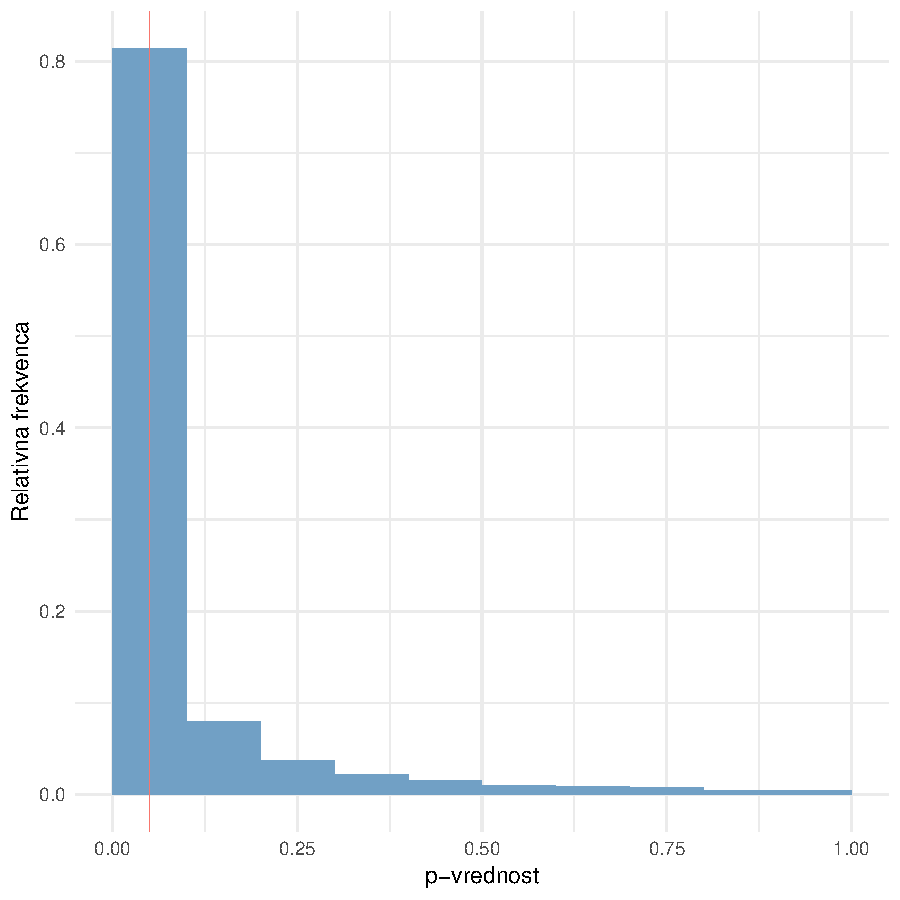
\includegraphics{zaplet_HA_M_Z7}
%    \subcaption{Zaplet 7 (beta = -0.8) - M}
%    \label{fig:1b}
%  \end{minipage}
%  \begin{minipage}[b]{.4\linewidth}
%    \centering
%    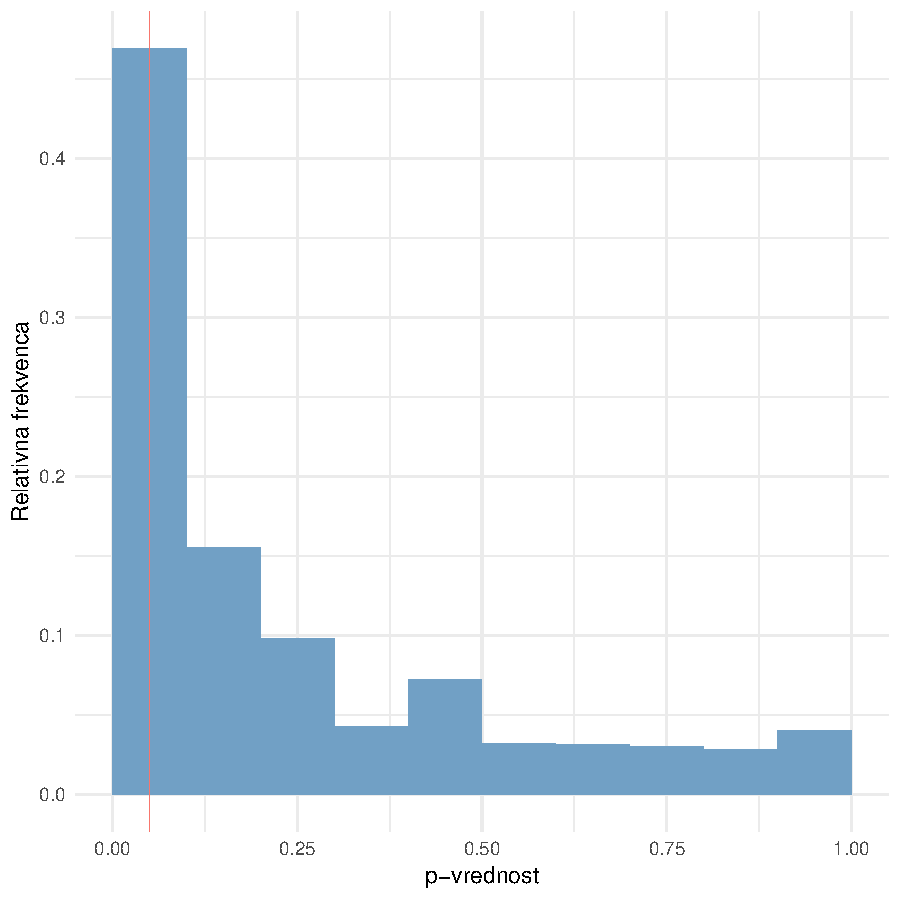
\includegraphics{zaplet_HA_U_Z8}
%    \subcaption{Zaplet 8 (beta = 0.6) - U}
%    \label{fig:1b}
%  \end{minipage}
%  \begin{minipage}[b]{.4\linewidth}
%    \centering
%    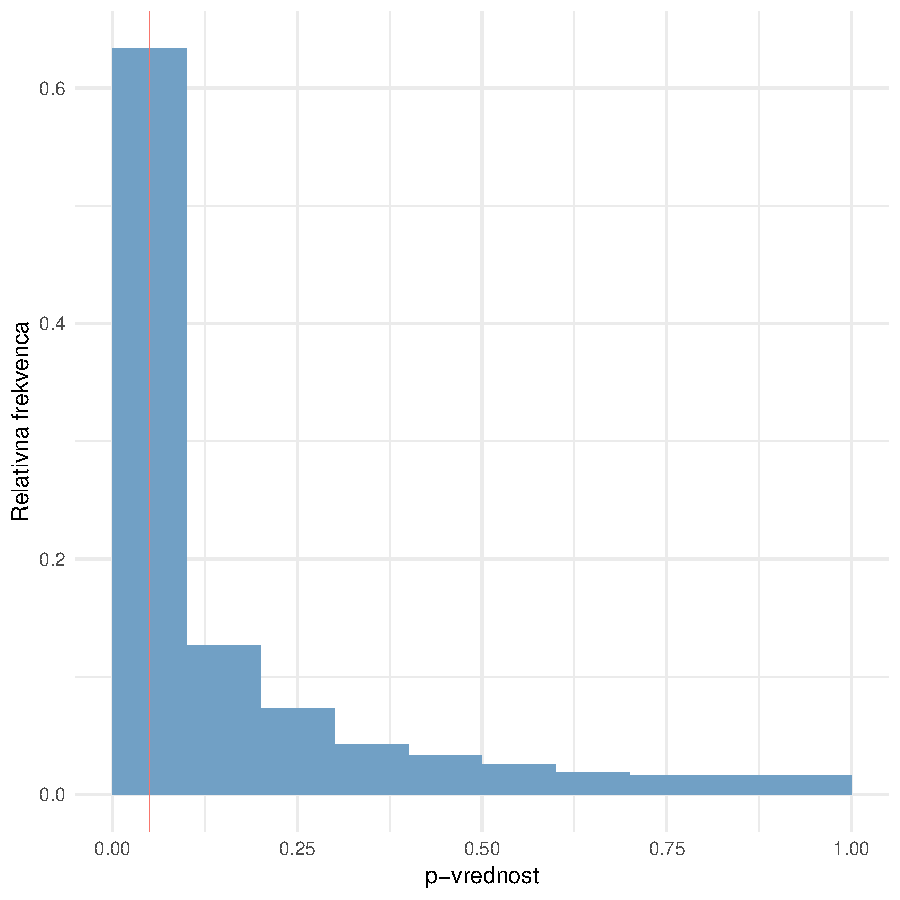
\includegraphics{zaplet_HA_M_Z8}
%    \subcaption{Zaplet 8 (beta = 0.6) - M}
%    \label{fig:1b}
%  \end{minipage}
%  \begin{minipage}[b]{.4\linewidth}
%    \centering
%    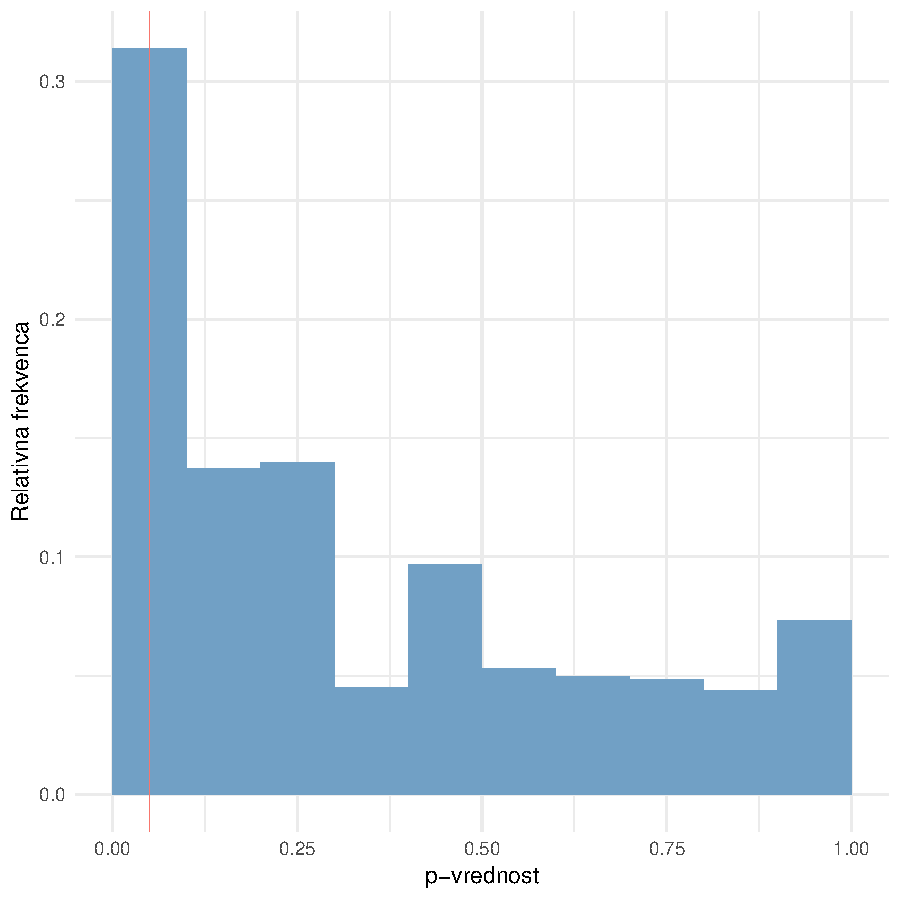
\includegraphics{zaplet_HA_U_Z9}
%    \subcaption{Zaplet 9 (beta = -0.4) - U}
%    \label{fig:1b}
%  \end{minipage}
%  \begin{minipage}[b]{.4\linewidth}
%    \centering
%    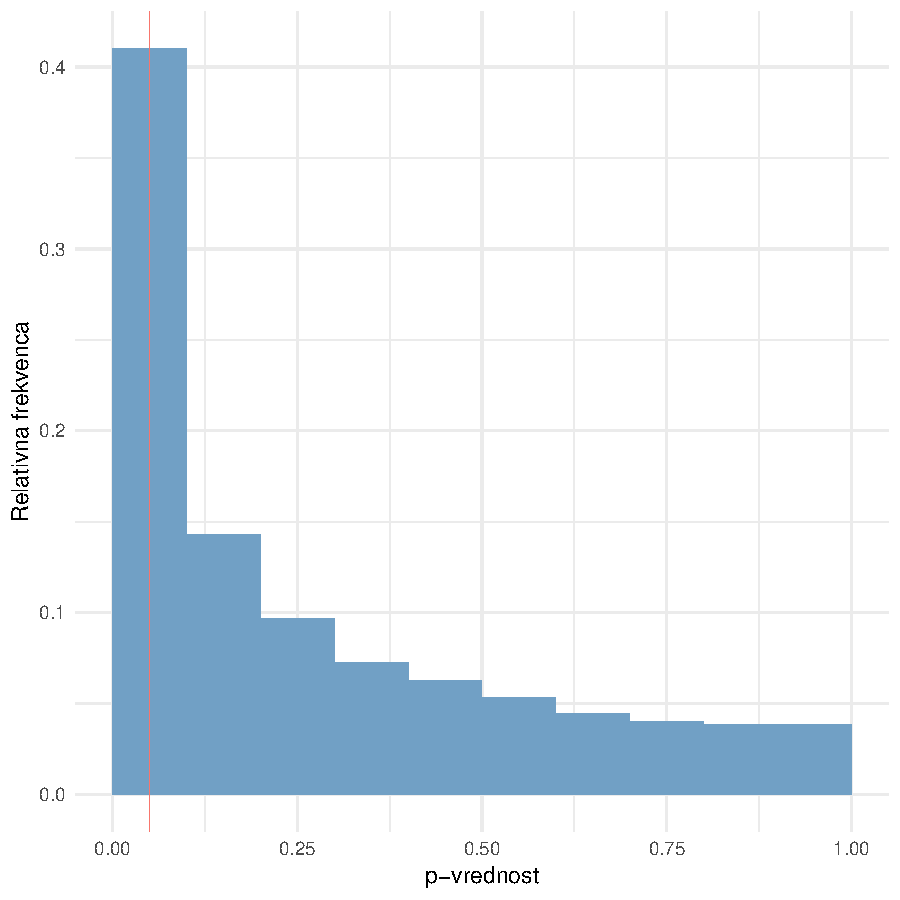
\includegraphics{zaplet_HA_M_Z9}
%    \subcaption{Zaplet 9 (beta = -0.4) - M}
%    \label{fig:1b}
%  \end{minipage}
%  \begin{minipage}[b]{.4\linewidth}
%    \centering
%    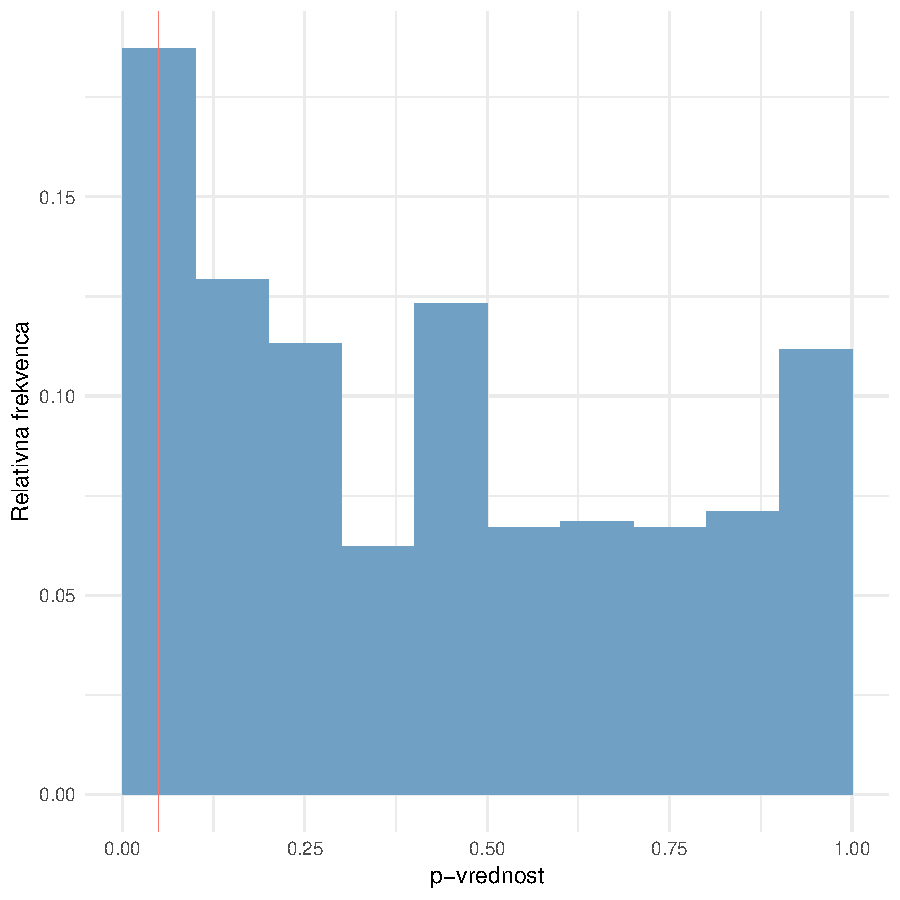
\includegraphics{zaplet_HA_U_Z10}
%    \subcaption{Zaplet 10 (beta = 0.2) - U}
%    \label{fig:1b}
%  \end{minipage}
%  \begin{minipage}[b]{.4\linewidth}
%    \centering
%    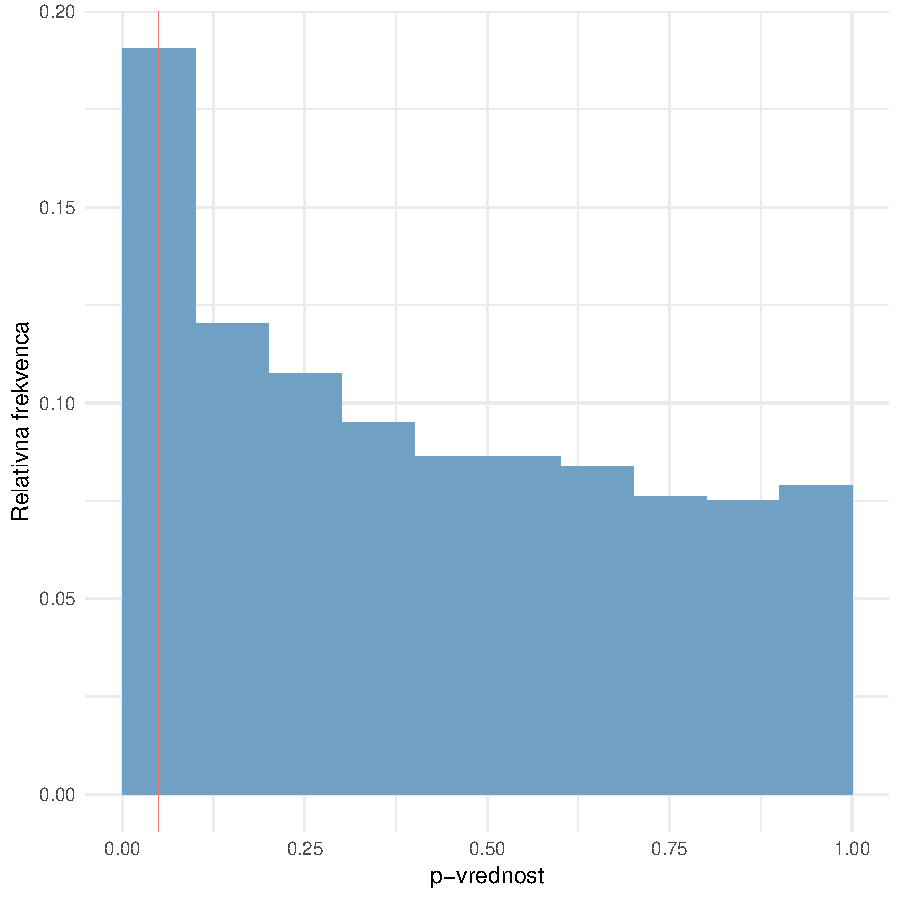
\includegraphics{zaplet_HA_M_Z10}
%    \subcaption{Zaplet 10 (beta = 0.2) - M}
%    \label{fig:1b}
%  \end{minipage}
%  \caption{Porazdelitve p-vrednosti pri HA gleda na zaplet in model (3/3)}
%  \label{fig:1}
%\end{figure}
%
\clearpage
\newpage
\section{Zaključek}

\end{document}
